\documentclass[modern]{aastex631}
\usepackage{amsmath}
\usepackage{amssymb}
\usepackage{hyperref}
\usepackage{bm}
\usepackage{listings}
\usepackage{graphicx}
\usepackage{float}

% commands
\newcommand{\nuancemethod}{\textit{nuance}}
\newcommand{\nuance}{\nuancemethod{}}
\newcommand{\nuancecode}{\textsf{nuance}}

\newcommand{\TODO}{\texttt{todo}}
\newcommand{\set}[1]{\{\,#1\,\}}
\newcommand{\footlink}[1]{\footnote{\url{#1}}}
\newcommand{\wtls}{\texttt{biweight+BLS}}
\DeclareMathOperator*{\argmax}{arg\,max}
\DeclareMathOperator*{\argmin}{arg\,min}

% no indent
\setlength\parindent{0pt}

% code style
\lstdefinestyle{mystyle}{
    backgroundcolor=\color{white},
    commentstyle=\color{gray!70},
    keywordstyle=\color{Bittersweet},
    stringstyle=\color{RoyalBlue},
    basicstyle=\fontsize{8.5}{13}\fontfamily{DejaVuSansMono-TLF}\selectfont,
    breakatwhitespace=false,         
    breaklines=true,
    rulecolor=\color{black!15},
    numbers=none,
    numberstyle=\fontsize{7}{11}\fontfamily{DejaVuSansMono-TLF}\selectfont\color{gray!50},
    framerule=0pt,
    breakindent=5pt,
    resetmargins=true,
    numbersep=10pt,
    frame=single,
    aboveskip=1em,
    belowskip=1em,
    xleftmargin=6pt,
    framexleftmargin=4pt
}
\lstset{style=mystyle}

% figure options
\graphicspath{{../figures}}

\begin{document}

\title{\texttt{nuance}: Detection of planetary transits in the presence of correlated noise}

% author info
\author{Lionel J. Garcia}
\author{Daniel Foreman-Mackey}
\affiliation{Center for Computational Astrophysics, Flatiron Institute, New York, NY, USA}
\author{Dax L. Feliz}
\author{Catriona A. Murray}
\correspondingauthor{Lionel J. Garcia}
\email{lgarcia@flatironinstitute.org}

\keywords{transit search, exoplanets, stellar activity, time series analysis, Gaussian processes}

\begin{abstract}
    We present \nuancemethod{}, an algorithm to search for planetary transits in light curves featuring correlated noise, such as instrumental signals and stellar photometric variability. To deal with them, a common approach consists in cleaning a light curve from nuisance signals before searching for transits. However, we show that this approach, based on the prior assumption that transits are not present, strongly degrades their signal-to-noise-ratio down to no detection. As this degradation depends on the correlated noise characteristics, we explore the relative parameter space for which transits are altered, and quantify this effect on a set of simulated light curves. On this synthetic dataset, we show that \nuancemethod{} largely outperforms the detection capabilities of a commonly used transit search technique, which consists in cleaning light curves from styellar variability with an optimal bi-weight filter before searching for transits using a box-least-square algorithm. Then, in order to assess the performance of \nuancemethod{} on real datasets, we inject and recover transits into the TESS light curves of 438 M dwarfs, and compare our method to 4 detrending techniques followed by a Box-Least-Square search. For transits with a duration exceeding one fifth of the stellar variability timescale, i.e. when both signals start resembling each other, we show that our algorithm is the most performant in 94\% of cases, leading to both the highest number of true positives and the lowest number of false positive detections. Although simultaneously searching for transits while modeling correlated noise is expected to be computationaly expensive, we make our algorithm tractable and available as the \textsf{JAX}-powered Python package \href{https://github.com/lgrcia/nuance}{\nuancecode{}}, allowing its use on distributed environments and GPU devices (?). Finally, we explore the prospects offered by the \nuancemethod{} formalism, and its use to advance our knowledge of active stars and their transiting exoplanets, both using space-based and sparse ground-based observations.
\end{abstract}


\section*{Introduction}
Transiting exoplanets are keystone objects for the field of exoplanetary science, but detecting transits in light curves featuring stellar variability and instrumental signals remains a challenge \citep{Pont2006,Howell2016}. For this reason, known transiting exoplanets tend to be found around quieter stars, or belong to the population of close-in giants whose transit signals dominate over stellar rotational variability \citep{Simpson2023}. However, discovering transiting exoplanets around active stars holds few promises. First, as younger stars are more active \citep{Skumanich1972}, being able to detect planets transiting active stars will favor the discovery of young planetary systems \citep[e.g.][]{Newton2022}. Second, as stellar variability may originate from surface active regions (such as starpots), the increased discovery of occulting companions will increase our chances to map the photosphere of active stars \citep[e.g.][]{Morris2017}, benefiting both the study of stellar atmospheres and the concerning impact of their non-uniformity on planetary atmosphere retrievals \citep{rackham2018}. Overall, enabling the detection of transits in light curves with high levels of correlated noises will greatly benefit the study of terrestrial exoplanets around late M-dwarfs, usually observed at lower SNR and more likely to display photometric variability (e.g. \citealt{Murray2020}).
\\\\
Commonly used transit-search algorithms, such as the Box-Least-Square algorithm \citep[BLS,][]{bls} are capable of detecting transits in light curves containing only transit signals and white noise. Using this method, the simplest way to detect transits in a light curve featuring correlated noise (either astrophysical or instrumental), is to first clean it from nuisance signals before performing the search. This strategy is widely adopted by the community, both using physically-motivated systematic models like \cite{everest1, everest2}, or filtering techniques (\citealt{Jenkins2010}, \citealt{wotan}). However, when correlated noise starts resembling transits, this cleaning step (often referred to as \textit{detrending}) is believed to degrade their detectability \cite[see subsection 4.3 of][]{wotan}. In this case, the only alternative to search for transits is to perform a full-fledged modeling of the light curve, including both transits and correlated noise, and to compute the likelihood of the data to the transit model on a wide parameter space (an approach largely avoided due to its intractable nature). Nonetheless, \cite{kovacs2016} ask: \textit{Periodic transit and variability search with simultaneous systematics filtering: Is it worth it?}. The latter study explores a handful of cases and generally discards the benefit of using a full-fledged approach. However, it does not explore the light-curves characteristics for which such a complete modeling becomes necessary.\\\\
In this paper, we explore the light curve characteristics for which a full-fledge transit search is necessary, and we present \nuancemethod{}\footnote{Throughout the paper, \nuancemethod{} written in italics refers to the algorithmic and analytical method, while \nuancecode{} in sans-serif refers to its implementation.}, a method to search for transit signals while modeling correlated noises in a tractable way. In \autoref{issues}, we describe the effect of correlated noise on transit light curves and the effect of its detrending on transit signals detectability. In \autoref{nuance}, we present \nuance{}, and the two main steps on which this method is based: the linear search and the periodic search. In \autoref{results}, we test the performance of \nuance{} on a wide variety of cases, and compare it to commonly used transit search algorithms. This include transits injected in synthetic datasets, but also in the TESS light curves of 438 rapidly-rotating M dwarfs. Finally, in \autoref{discussion}, we discuss the results and the limitations of \nuance{}, and we conclude in .

\newpage
\section{The issue}\label{issues}

A strong assumption when using the BLS algorithm to search for transits is that the searched dataset only contains these signals in addition of white noise. Hence, two sources of correlated noise particularly justify the need for a detrending step before searching for transits: instrumental signals (such as those induced by telescope pointing errors) and astrophysical signals (such as stellar variability induced by pulsations or starspots). In this section, we qualitatively study the effect of correlated noise and its detrending on transits detectability.

\subsection{Transit detectability}

One way to study the detectability of a unique transit signal is to compute its signal-to-noise-ratio (SNR, \citealt{Pont2006}, Equation 12):
\begin{equation}\label{eq:snr}
  SNR= \frac{\Delta}{\sqrt{\frac{\sigma_w^2}{n} + \frac{\sigma_c^2}{N_{tr}}}}
\end{equation}
where $\Delta$ is the relative transit depth, $n$ is the number of points within transit, $N_{tr}$ the number of transits ($N_{tr}=1$ here), and $\sigma_w^2$ and $\sigma_c^2$ are the white and correlated noise variances\footnote{i.e. $\sigma_w^2 = \sum_{i=j} C_{{ij}}$ and $\sigma_c^2 = \sum_{i\neq j} C_{{ij}}$ with $C$ the covariance matrix of the data.}. \autoref{fig:issue1} shows this metric computed for a unique transit observed in the absence (grey) and presence (red) of correlated noise.

\begin{figure}[H]
    \begin{centering}
        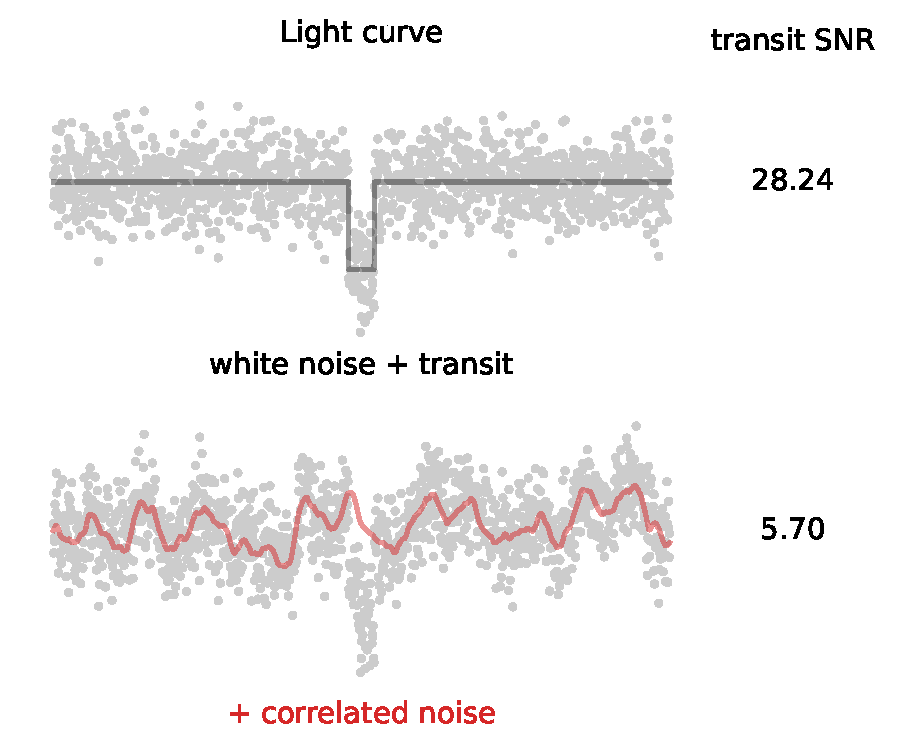
\includegraphics[width=0.6\linewidth]{../workflows/plot_issues/figures/issue1.pdf}
        \caption{Illustration of the effect of correlated noise on a single transit SNR. A 1-hour transit signal of depth 1\% is generated on top of white noise (variance of $0.0015^2$) as part of a 24-hours observation with an exposure time of 1 minute (top). Then, in the bottom plot, correlated noise is added, generated using a Gaussian process (GP; \citealt{Rasmussen2005}) with a Matèrn-32 kernel of scale 1 hour and sigma of 0.2\%. The SNR on the right of each light curve is computed using \autoref{eq:snr}. Models used to simulate these data are provided in \autoref{signals_simulations}.}
        \label{fig:issue1}
    \end{centering}
\end{figure}

As illustrated in \autoref{fig:issue1}, the presence of correlated noise strongly decreases the transit signal SNR, which would ultimately limit its detectability.

\subsection{Detrending methods and their effects}\label{detrending_effect}
The presence of instrumental correlated noise motivated the development of systematics detrending algorithms, such as the Trend Filtering Algorithm (\textsc{TFA}, \citealt{tfa}, in its primary use case), \textsc{SysRem} (\citealt{sysrem}) or Pixel Level Decorrelation (\textsc{PLD}, \citealt{pld}; see also \textsc{Everest} from \citealt{everest1, everest2}). Most of these methods rely on the shared nature of instrumental signals among light-curves (or neighboring pixels) such that the correction applied should not degrade the transit signal and can be modeled using contemporaneous measurements (like detector's temperature, pointing error, sky background or airmass time series).
\begin{figure}[H]
    \begin{centering}
        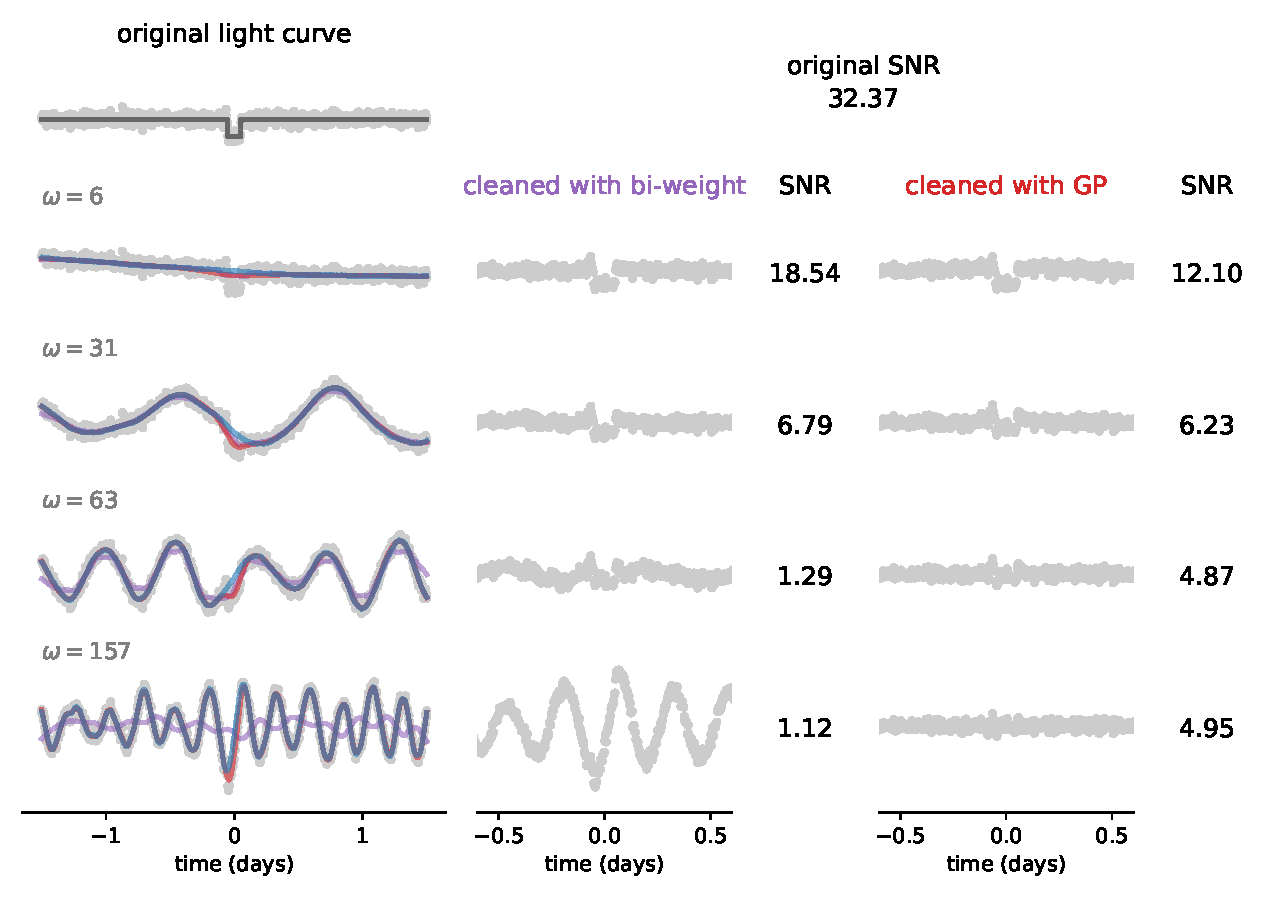
\includegraphics[width=\linewidth]{../workflows/plot_issues/figures/issue2.pdf}
        \caption{(Top left) Simulated observation spanning 3 days, including a transit signal with a depth of 0.8\%, duration of 0.1 day, and measurement error of 1.5\% (using the model from \cite{protopapas} described in \autoref{app_proto}). (Left) Correlated noise in the form of stellar variability with different timescales and amplitudes added to the unique transit signal. This signal is then reconstructed using (in purple) Tukey's bi-weight filter \citep{wotan} with an optimal window size of three times the transit duration, and (in red) a GP with the same kernel used to simulate the data. In each case the variability is reconstructed, subtracted, and the transit SNR computed using \autoref{eq:snr} with the transit depth estimated as the minimum in-transit flux.}
        \label{fig:issue2}
    \end{centering}
\end{figure}
In opposition, stellar variability and other astrophysical signals cannot be correlated with simultaneous measurements. This gave rise to several treatments in order to reconstruct and detrend stellar variability. Some of them are physically-motivated and make use of GPs (e.g. \citealt{k2sc}), others are empirical and make use of filtering and data-driven algorithms (\citealt{Jenkins2010}, \citealt{wotan}).\\\\
In \autoref{fig:issue2}, we simulate a transit signal on top of which we add photometric stellar variability with different amplitudes and timescales, sampled from a GP with an SHO kernel described in \autoref{app_gp}. For each light curve, we reconstruct and detrend stellar variability in two ways: one using the widely-adopted Tukey's bi-weight filter, presented in \cite{tukey} and using the implementation from \textsf{wõtan}\footnote{\href{https://github.com/hippke/wotan}{https://github.com/hippke/wotan}} \citep{wotan}; the other using the same GP from which the data has been sampled. We then estimate the resulting transit depth and compute the remaining transit SNR using \autoref{eq:snr}. \autoref{fig:issue2} clearly shows the effect of both detrending techniques on transits SNR, and intuitively suggests that this degradation due to detrending is strongly dependant on the correlated noise characteristics encountered.\\\\
In order to explore the parameter space for which detrending is the most problematic, we employ the method previously described to simulate 10 000 light curves containing a transit signal and correlated noise in the form of stellar variability. For each light curve, we reconstruct the variability signal and detrend it using an optimal bi-weight filter, i.e. with a window size three times that of the transit duration \citep{wotan}, before estimating the remaining transit SNR. For convenience, the simulated light curves share a common transit added on top of white noise, and a variability signal only defined by two parameters: $\tau$, the relative timescale of the variability with respect to the transit duration; and $\delta$, the relative amplitude of the variability against transit depth, corresponding to an SHO kernel with hyperparameters chosen as: 
\begin{equation}\label{eq:relative_params}
    \omega = \frac{\pi}{\tau D}, \hspace{0.5cm} 
    \sigma = \delta \frac{\Delta}{2} \hspace{0.5cm}  \text{and}  \hspace{0.5cm}  
    Q = 10,
\end{equation}
with $\Delta=1\%$ and $D=0.04$ days, the depth and duration of the simulated transit. 
% We fix a relatively high value for the quality factor $Q$ in order to restrict our simulations to strongly periodic variability signals. 

For $\tau=1$ and $\delta=1$, the expressions of $\omega$ and $\sigma$ given in \autoref{eq:relative_params} correspond to a variability signal with a period half that of the transit duration, and a correlated noise amplitude comparable to the transit depth, i.e. strongly resembling the simulated transit signal.\\\\
\autoref{fig:snr_detrend} shows that it exists an entire region of the $(\tau, \delta)$ parameter space for which the bi-weight detrending degrades transit SNR to the point of no detection ($SNR < 6$). Hence, bi-weight filter detrending makes transit search blind to many systems. While this study should be extended to other detrending techniques, it highlights the need for a more informed transit search algorithm able to deal with correlated noise, at least if present in the form of stellar variability.

% ## STOPPED here


\begin{figure}[H]
    \begin{centering}
        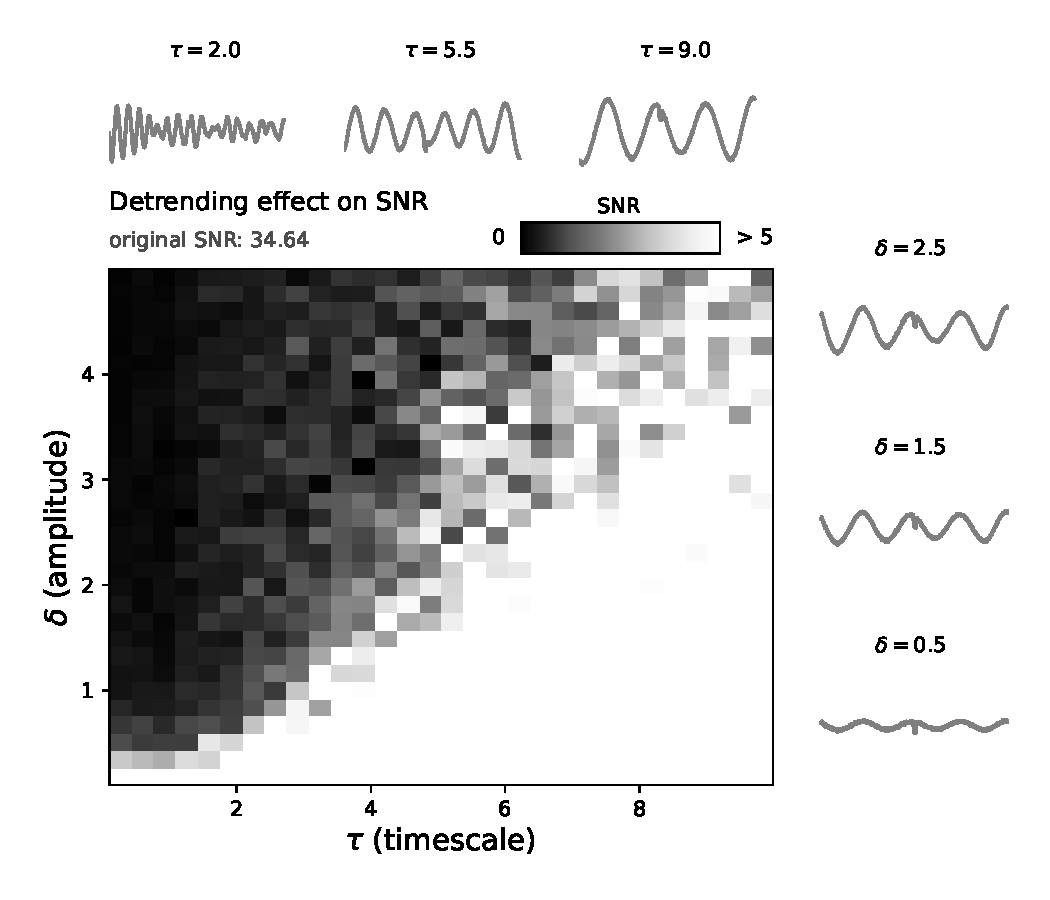
\includegraphics[width=0.9\linewidth]{../workflows/cleaning_snr/figures/result.pdf}
        \caption{SNR of a unique transit after detrending light curves using an optimal bi-weight filter (i.e.\;of window size $3\times D$). All light span 2.8 days with exposure times of 2 minutes. The 10 000 simulated datasets contain the same transit signal with a duration $D=1$ hour and a depth of 1\%, added on top of white noise with a standard deviation of 0.5\% plus stellar variability. Light curves at the top and right side of the central plot are shown with their corresponding $\tau$ and $\delta$ values, which again correspond to the relative timescale of stellar variability against the transit duration, and the relative amplitude of stellar variability against the transit depth. Hence, the amplitude of the variability increases with $\delta$ and the timescale of the variability increases with $\tau$, the transit signal remaining fixed.}
        \label{fig:snr_detrend}
    \end{centering}
\end{figure}


\newpage
\section{\textsf{nuance}}\label{nuance}

\textit{nuance} is an algorithm capable of searching for planetary transits in light curves containing correlated noise, such as instrumental signals and photometric stellar variability.
\\\\
Let assume that the flux $f$ of a star is observed and arranged in the vector $\bm{f}$ of size $N$, associated to the vector of times $\bm{t}$. This flux, shown in \autoref{fig:linear_search}, contains instrumental signals, stellar variability and a periodic transit signal that we wish to detect. We assume that a set of $M$ observed measurements (such as the position of the star on the detector or the sky background) taken at the same time as the flux can be treated as explanatory variables for $\bm{f}$. These measurements constitute the columns of the $(N\times M)$ \textit{design matrix} $\bm{X}$.\\\\
Ideally, we would detect the periodic transit signal in this flux by sampling the posterior likelihood of this data to a full-fledge model including stellar variability (more generally correlated noise), instrumental systematic signals (modeled with explanatory variables or treated as correlate noise), and a periodic transit signal of period $P$, epoch $T_0$, duration $D$ and depth $\Delta$. We would then reduce the posterior likelihood to $p(\bm{f}\vert P)$, its marginalized version over all parameters except the period $P$, producing a transit search periodogram $\mathcal{Q}(P)$. However, this approach has two issues: It is highly intractable, and it may lead to a multimodal distribution that is hard to interpret.
\\\\
Given a period $P$, we instead want to compute the likelihood of a periodic transit signal at the maximum likelihood parameters $\hat T_0$, $\hat D$ and $\hat \Delta$, i.e the periodogram
\begin{equation}\label{eq:periodogram}
        \mathcal{Q}(P) = p(\bm{f} \vert P, \hat T_0 ,\hat D, \hat \Delta)
\end{equation}
This is done by adopting the strategy of \cite{foreman2016}, separating the transit search into two components: the linear search and the periodic search. During the linear search, the likelihood of a single non-periodic transit is computed for a grid of epochs, durations and depths. Then, the periodic search consists in combining these likelihoods to compute the likelihood of the data given a periodic transit signal for a range of periods. These combined likelihoods yield a transit-search periodogram on which the periodic transit detection is based. \textsf{nuance} differs from \cite{foreman2016} and other existing transit search algorithms as it models the covariance of the light curve with a GP, accounting for correlated noise (especially in the form of stellar variability) while keeping the model linear and tractable. This way, \textsf{nuance} searches for transits while, at the same time, modeling correlated noise, avoiding the detrending step that degrades transit signals SNR.\\\\
We note that the approach employed by \nuancemethod{} (using the two steps proposed by \citealt{foreman2016}), shares similarities with the approach of \cite{Jenkins2010}, where a single event statistic is computed and combined into a multiple event statistics.

\subsection{The linear search}\label{linear_search}

The goal of the linear search is to compute the likelihood $p(\bm{f} \vert T , D, \Delta)$ of the data given a single non-periodic transit signal of epoch $T$, duration $D$ and depth $\Delta$, for a grid of epochs, durations and depths.
\\\\
To account for correlated noise, the light curve $f$ is modeled as being drawn from a GP, like the simulated light curves used in \autoref{issues}, such that
\begin{equation*}
    \bm{f} \sim \mathcal{N}(\bm{X w}, \bm{\Sigma}),
\end{equation*}
with mean $\bm{Xw}$ (i.e. a linear model of the M explanatory variables with coefficients $\bm{w}$) and covariance $\bm{\Sigma}$. To account for the presence of a single non-periodic transit of epoch $T$ and duration $D$, this signal is computed and appended as the last column of the design matrix $\bm{X}$, using the simple transit model from \cite{protopapas} with a unitary depth (\autoref{eq:protopapas}). This way, the transit signal is part of the linear model and its depth $\Delta$ can be solved linearly. Under this assumption, the log-likelihood of the data given a single non-periodic transit is \citep{Rasmussen2005}
\begin{equation} \label{eq:linear_search_ll}
    \ln p(\bm{f} \vert I) = -\frac{1}{2}(\bm{f}-\bm{Xw})^T\bm{\Sigma}^{-1}(\bm{f}-\bm{Xw}) -  \frac{1}{2}\ln\vert\bm{\Sigma}\vert - \frac{N}{2}\ln 2\pi,
\end{equation}
where the parameters vector $\bm{w}$ and their errors $\bm{\sigma}$ are computed using the generalized least-square solution
\begin{equation}\label{eq:ls}
    \bm{w} = (\bm{X}^T\bm{\Sigma}^{-1}\bm{X})^{-1}\bm{X}^T\bm{\Sigma}^{-1}\bm{f} \hspace{0.5cm} \text{and} \hspace{0.5cm} \bm{\sigma} = (\bm{X}^T\bm{\Sigma}^{-1}\bm{X})^{-1},
\end{equation} 
with $\bm{\Sigma}$ the covariance matrix modeled using the GP. Hence, $\ln p(\bm{f} \vert I)$ can be computed on a grid of epochs and durations, the transit depth being linearly solved for any $(T, D)$. This \textit{linear search} leads to the set of likelihoods
\begin{equation*}
    \set{\ln\mathcal{L}_{i,j}}_{i, j} = \set{\ln p(\bm{f} \vert T_i ,D_j, \Delta_{i,j})}_{i, j},
\end{equation*}
were $\Delta_{i,j}$ is the depth linearly solved for a given $(T_i, D_j)$\footnote{The expression of $\set{\ln\mathcal{L}_{i,j}}_{i, j}$ omits the vector $\bm{w}_{i,j}$ (except its last value $\Delta_{i,j}$) as it is also linearly solved for any given value of $(T_i, D_j)$ and irrelevant in what follows.}. \autoref{fig:linear_search} shows this likelihood grid computed for a simulated dataset, using the same GP  and design matrix $\bm{X}$ used to simulate the data.

\begin{figure}[H]
    \begin{centering}
        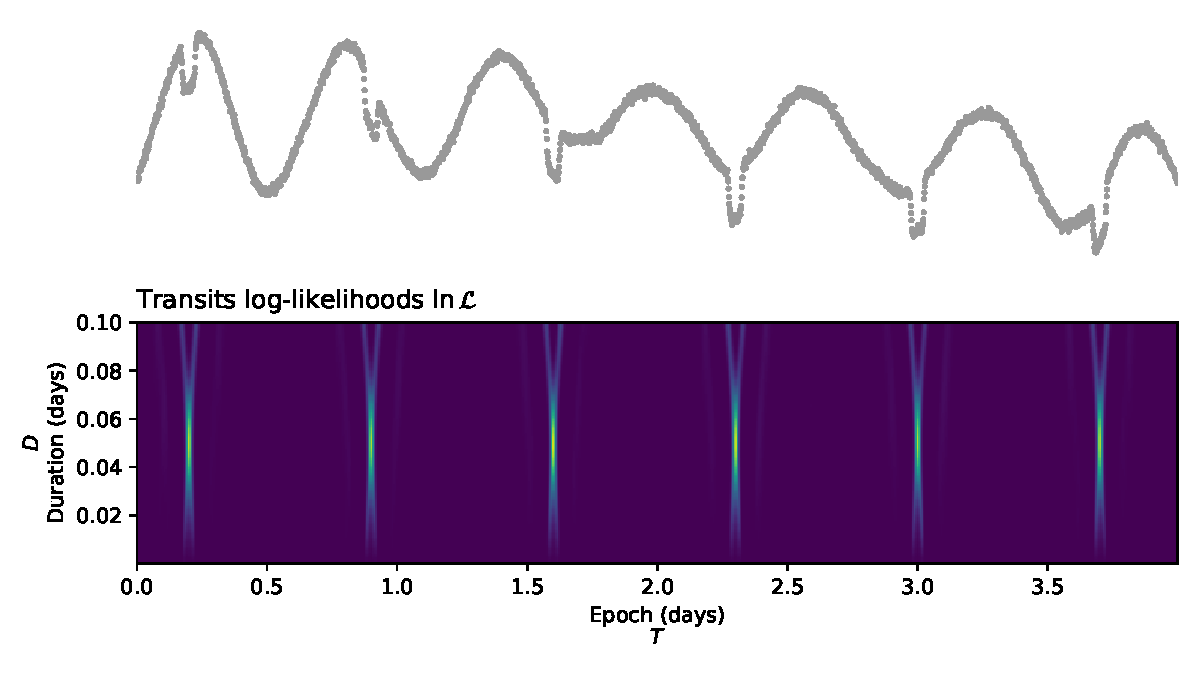
\includegraphics[width=\linewidth]{../workflows/principle/figures/principle_linear_search.pdf}
        \caption{Principle and output of the linear search. The simulated dataset (top) corresponds to the one shown and described in \autoref{fig:app_principle_dataset}. First, a set of durations and depths $\set{T_i, D_j}_{i,j}$ is generated. For each pair of indices $(i,j)$, the likelihood $\ln p(\bm{f} \vert T_i ,D_j, \Delta_{i,j})$ is computed using the parameters from \autoref{eq:ls} and the expression of \autoref{eq:linear_search_ll}. This process yields the grid of log-likelihoods $\ln\mathcal{L}$ (bottom plot), as well as the $\set{\Delta_{i,j}, \sigma_{i,j}}_{i, j}$ transit depths and errors inferred linearly using \autoref{eq:ls}.}
        \label{fig:linear_search}
    \end{centering}
\end{figure}

\noindent To prepare for the next step, the corresponding depths $\Delta_{i,j}$ linearly solved for any $(T_i ,D_j)$ are stored, as well as their associated uncertainties $\sigma_{i,j}$, corresponding to
\begin{equation*}
    \Delta_{i,j} = \bm{w}_M \hspace{0.5cm}\text{and}\hspace{0.5cm} \sigma_{i,j} = \bm{\sigma}_{MM},
\end{equation*}
M denoting the index of the last column of the design matrix $\bm{X}$, where the transit signal is contained.

\subsection{The periodic search}

We then need to combine the likelihoods computed from the \textit{linear search} to obtain
\begin{equation*}
    p(\bm{f} \vert P, T_0 , D, \Delta),
\end{equation*}
i.e.\,the probability of a periodic transit of period $P$, epoch $T_0$, duration $D$ and depth $\Delta$ given the data $\bm{f}$. For a given transit duration $D$, any combination of $(P, T_0)$ leads to K transits, for which it is tempting to write
\begin{equation}\label{eq:attempt}
    p(\bm{f} \vert P, T_0 ,D, \Delta) = \prod_k^K p(\bm{f} \vert T_k, D, \Delta_k),
\end{equation}
where $\set{T_k}_k$ are the epochs matching $(T_0, P)$ and $\set{\Delta_k}_k$ the corresponding depths. So that
\begin{equation*}
    \ln p(\bm{f} \vert P, T_0 ,D, \Delta) = \sum_k^K \ln \mathcal{L}_k.
\end{equation*}
This is the joint likelihood of transits belonging to the same periodic signal but with varying depths  $\set{\Delta_k}_k$. However, individual transits from a periodic signal cannot be considered independent, and should instead be found periodically and share a common transit depth $\Delta$. To this end, it can be shown (see \autoref{proof}) that there is an analytical expression for the joint likelihood of K individual transits with depths and errors $\set{\Delta_k, \sigma_k}_k$ assuming a common depth $\Delta$, corresponding to 
\begin{equation}\label{eq:result}
    \begin{gathered}
        \ln p(\bm{f} \vert P, T_0 ,D, \Delta) =  \sum_{k}^K \ln \mathcal{L}_k  - \frac{1}{2} \sum_k^K\left(\ln(\sigma_{k}^2) - \ln(\sigma^{2} + \sigma_{k}^{2}) +  \frac{\left(\Delta_{k} -
        \Delta\right)^{2}}{\sigma_k^{2} + \sigma^{2}}\right) \\
        \text{with} \quad  \frac{1}{\sigma^2} = \sum_k^K \frac{1}{\sigma_k^2} \quad \text{and} \quad
        \Delta = \sigma^2 \sum_k^K {\frac{\Delta_k}{\sigma_k^2}}.
    \end{gathered}
\end{equation}

While \autoref{eq:result} takes a closed form, the individual epochs matching $T_0$ and $P$ are not necessarily available in the grid of epochs $\set{T_k}_k$. In \cite{foreman2016}, a similar issue is solved by using the nearest neighbors in the epochs grid. Instead, to allow the efficient matrix computation of \autoref{eq:result}, the likelihood grid is linearly interpolated from $\set{T_i}_i$ to a common grid of transit phases $\set{\phi_i}_i$, leading to the periodic search log-likelihood
$$\ln\mathcal{P}(P) = \set{\ln p(\bm{f} \vert P, \phi, D)}_{i,j}$$
shown for few periods in \autoref{fig:periodic_search} (b). In the latter equation, $\Delta_{i,j}$ is omitted since being interpolated from the linear search using $\phi_i$, $D_j$ and $T_0 = 0$.

\begin{figure}[H]
    \centering
    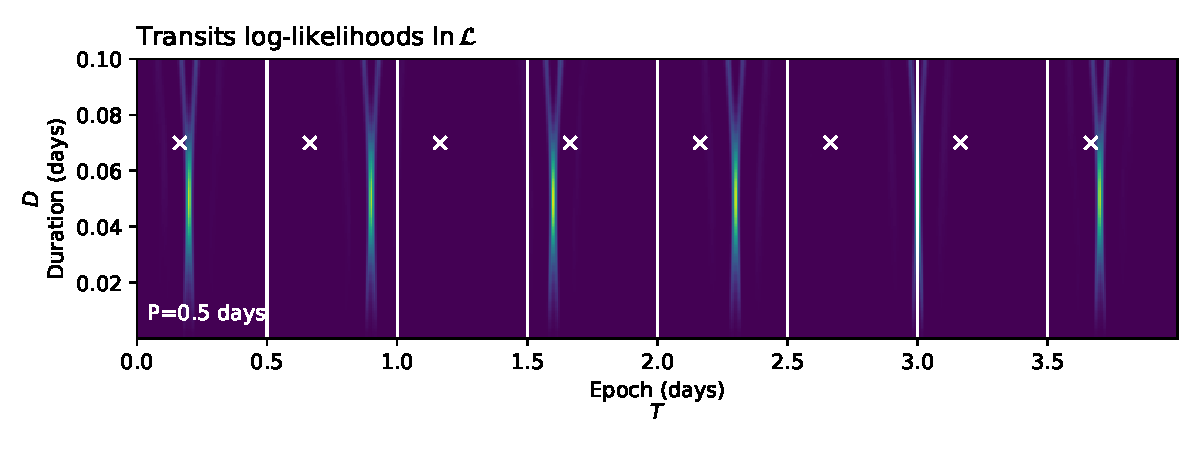
\includegraphics[width=\linewidth]{../workflows/principle/figures/principle_periodic_0.pdf}\\
    {(a) $\ln \mathcal{L}$}
\end{figure}

\begin{figure}[H]
    \centering
    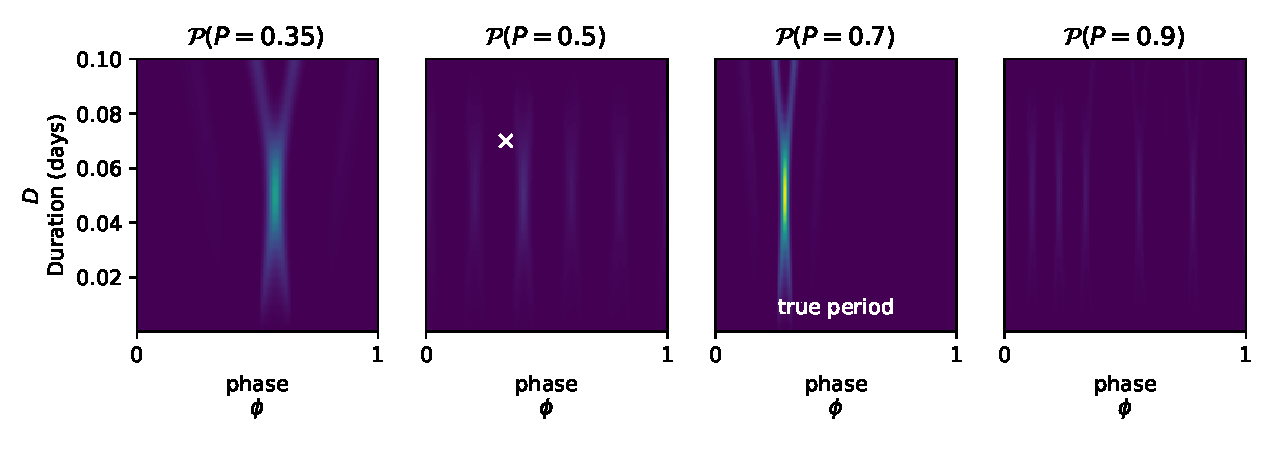
\includegraphics[width=\linewidth]{../workflows/principle/figures/principle_periodic_1.pdf}\\
    {(b) $\mathcal{P}(P)$}

    \caption{Applied to the dataset shown in \autoref{fig:linear_search}, this figure shows how the periodic search works at different periods $P$ (including the true period $P = 0.7$ days). Given different periods $P$ and $T_0=0$, the likelihood $\ln\mathcal{L}$ shown in (a) is phase-folded and interpolated onto a common grid of phases shown in (b). As an example, the white lines in (a) mark the edges of each fold for a period $P=0.5$ days, and the white crosses show the epochs $\set{T_k}_{k\in\mathbb{K}}$ matching a particular phase in the grid (reported in (a) and (b)) on which the corresponding $\set{\ln \mathcal{L}_k}_{k\in\mathbb{K}}$ are interpolated and combined using \autoref{eq:result}. To allow the use of efficient matrix computations, this is done for all durations $\set{D_i}_i$ so that $\mathcal{P}$ is computed on the full grid $\set{D_i, \phi_i}_{i, j}$ at once. We understand from the folded likelihoods plots in (b) that a different choice of epoch $T_0$ may only shift the results in phase but do not affect the values of $\mathcal{P}$. For this reason, computing $\mathcal{P}$ for $T_0=0$ is sufficient. We also notice how the maximum value of $\mathcal{P}(P=0.7/2)$ (left plot of (b)) is lower than for $P=0.7$ days, a result of combining the log-likelihoods using \autoref{eq:result} instead of \autoref{eq:attempt}, in favor of individual transits matching a common depth $\Delta$.}
    \label{fig:periodic_search}
\end{figure}

\subsection{The transit search periodogram}

Using \autoref{eq:result}, we can now compute $\ln\mathcal{P}$ for a range of periods and build a transit search periodogram using \autoref{eq:periodogram}. But a final issue emerges, one that is fundamentally linked to our strategy. Each likelihood $p(\bm{f} \vert T, D, \Delta)$ estimated during the linear search is computed using N measurements. Hence, combining transits in the periodic search, through $\Delta_k$, $\sigma_k$ and the product of $K$ likelihoods $\set{\mathcal{L}_k}_k$ (see \autoref{eq:result}), artificially leads to a likelihood involving $N\times K$ measurements. This lead to a normalization issue when trying to compare the joint log-likelihoods $\mathcal{P}(P)$ from one period to another, as the number of observed transits differs from one period to another. This motivates a final step to produce the transit search periodogram $\mathcal{Q}$. For any period P, instead of taking $ \mathcal{Q}(P)$ as the maximum value of $\ln\mathcal{P}$, we compute the maximum likelihood parameters
\begin{equation}\label{eq:phi0}
    (\phi_0 ,D) = \argmax_{\phi_i, D_j} \set{\ln p(\bm{f} \vert P, \phi_i, D_j)}_{i, j}
\end{equation}
and defined $\mathcal{Q}(P)$ as being equal to the SNR of the transit of period $P$, epoch $T_0 = \phi_0 P$, duration $D$ and depth $\Delta$, i.e.
\begin{equation*}
    \mathcal{Q}(P) = \frac{\Delta}{\sigma},
\end{equation*}
where $\Delta$ and $\sigma$ are obtained using \autoref{eq:sigma_delta} with the last column of $X$ containing a periodic transit signal of period $P$, epoch $T_0$, duration $D$ and depth $1$. This process and the resulting periodogram $\mathcal{Q}$ are shown in \autoref{fig:periodogram}.
\begin{figure}[H]
    \begin{centering}
        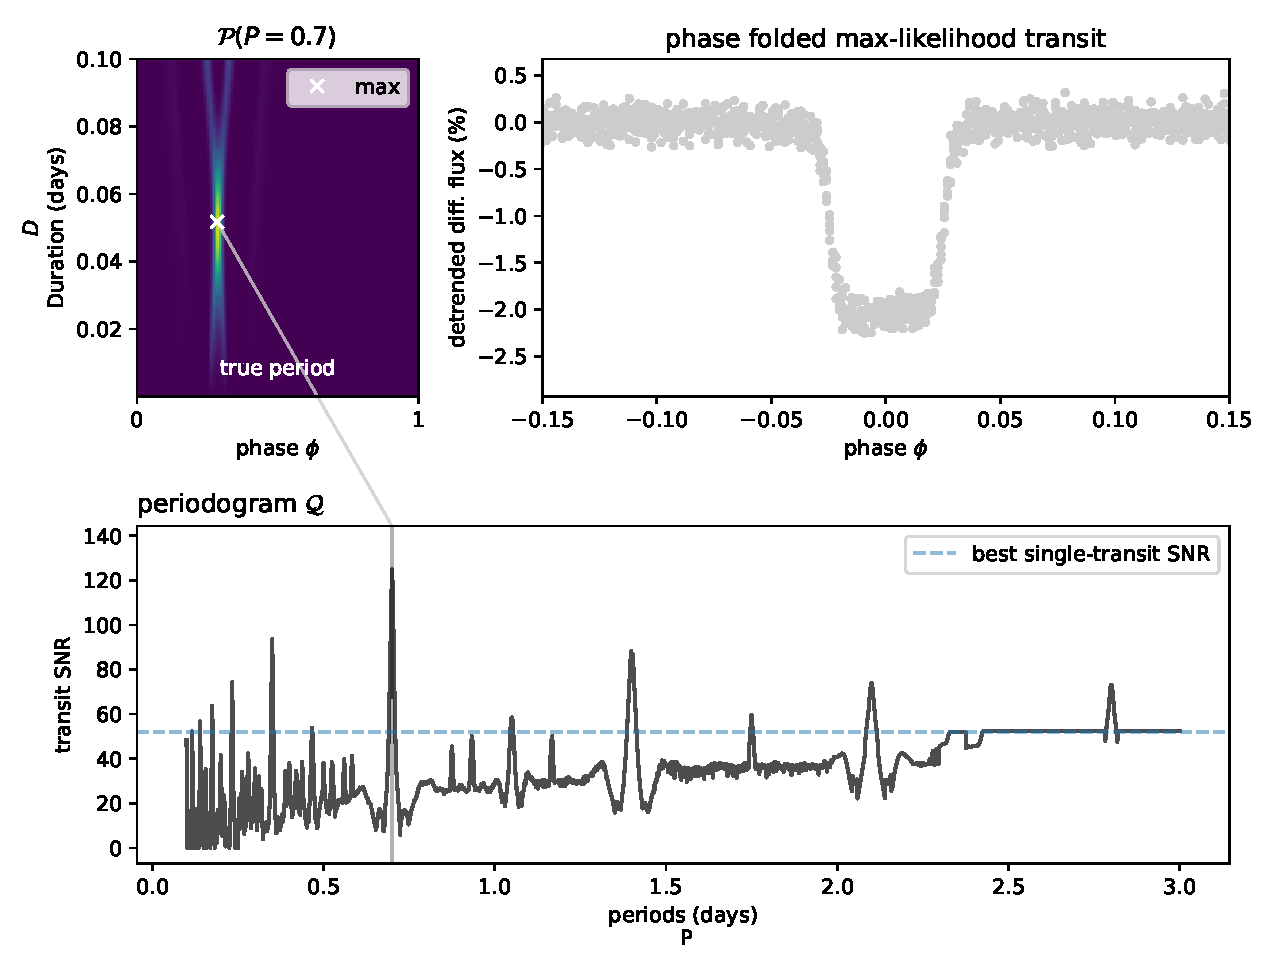
\includegraphics[width=\linewidth]{../workflows/principle/figures/principle_Q.pdf}
        \caption{For each period $P$, the joint likelihood $\mathcal{P}(P)$ is computed using \autoref{eq:result}, and the value of the maximum likelihood transit SNR retained as $\mathcal{Q}(P)$.}
        \label{fig:periodogram}
    \end{centering}
\end{figure}
The periodic transit of period $P$ with the maximum SNR, i.e. maximizing $\mathcal{Q}$, is adopted as the best candidate, basing the confidence in this signal through its SNR. The parameters of this transit are the period $P$, the epoch $T_0 = \phi_0 P$ and duration $D$ (\autoref{eq:phi0}), and the depth $\Delta$ with error $\sigma$ (given by \autoref{eq:result}).

\subsection{An open-source python package}
Methods presented in this paper are made accessible through the \nuancecode{} open-source Python package, hosted on Github\footnote{\href{https://github.com/lgrcia/nuance}{https://github.com/lgrcia/nuance}} and released on the Python Package Index\footlink{https://pypi.org/project/nuance/}. 
\\\\
To instantiate a search, a user can start by creating a \textsf{Nuance} object with
\begin{lstlisting}[language=Python]
from nuance import Nuance

nu = Nuance(time, flux, gp=gp, X=X)
\end{lstlisting}
where \textsf{gp} is a \textsf{tinygp} GP instance and \textsf{X} the design matrix of the linear model. \textsf{nuance} exploits the use of \textsf{tinygp}\footnote{\href{https://github.com/dfm/tinygp}{https://github.com/dfm/tinygp}}, a Python package powered by \textsf{JAX}\footnote{\href{https://github.com/google/jax}{https://github.com/google/jax}}, allowing for custom kernels to be built and highly tractable computations. We can then define a set of epochs \textsf{t0s} and durations \textsf{Ds} and run the linear search with
\begin{lstlisting}[language=Python,linewidth=\linewidth]
import numpy as np

t0s = time.copy()
# a range of 10 durations
Ds = np.linspace(0.01, 0.2, 10)
nu.linear_search(t0s, Ds)
\end{lstlisting}
Finally, the periodic search is run with
\begin{lstlisting}[language=Python]
# range of periods
periods = np.linspace(0.1, 5, 2000)
search = nu.periodic_search(periods)
\end{lstlisting}
From this \texttt{search} object, the best transiting candidate parameters can be computed (\textsf{search.best}), or the $\mathcal{Q}$ periodogram retrieved (\textsf{search.Q\_snr}), together with valuable information about the transit search. The \textsf{Nuance} object also provides methods to perform transit search on light curves from multi-planetary hosts, the advantage of \nuancemethod{} being that the linear search only needs to be performed ones and reused for the search of several transiting candidates (cf.\;\autoref{toi540}). An extensive and maintained online documentation is provided at \href{https://nuance.readthedocs.io}{\texttt{nuance.readthedocs.io}}.

\subsection{Comparison with BLS}\label{control}

To start testing \nuancemethod{} against existing methods, a simple adimensional normalized light curve is simulated, consisting in pure white noise with a standard deviation of $5\times 10^{-4}$ spanning 6 days with an exposure time of 2 minutes.
From this signal, we produce 4000 light curves, each containing box-shaped transits with periods randomly sampled from 0.3 to 2.5 days, durations of 50 minutes, and depths randomly sampled to lead to transit SNRs ranging from 4 to 30.
% (i.e.\;depths from $2.6 \times 10^{-4}$ to $6.8 \times 10^{-4}$, using the simple model from \cite{protopapas} presented in \autoref{app_proto} with $c=500$). By design, these injected signals have an SNR ranging from 5 to 30 (with $\sigma_r = 0$ in \autoref{eq:snr}). 
For each light curve, transits are searched using two different tools: \textsf{nuance}, using its implementation from the Python package described in the previous section; and BLS, the Box-Least-Square algorithm from \cite{bls} (using \textsf{astropy}'s \textsf{BoxLeastSquares}\footlink{https://docs.astropy.org/en/stable/api/astropy.timeseries.BoxLeastSquares.html} implementation).\\\\
For both methods, 3000 trial periods from 0.2 to 2.6 days are searched, with a single trial duration fixed to the unique known duration of 50 minutes. A transit signal is considered detected if the absolute difference between the injected and the recovered period is less than 0.01 day. To ease the detection criteria, orbital periods recovered at half or twice the injected ones (aka \textit{aliases}) are considered as being detected. For this reason, detected transit epochs are not considered (although manually vetted). Results from this \textit{injection-recovery} procedure are shown in \autoref{fig:control}.

\begin{figure}[H]
    \begin{centering}
        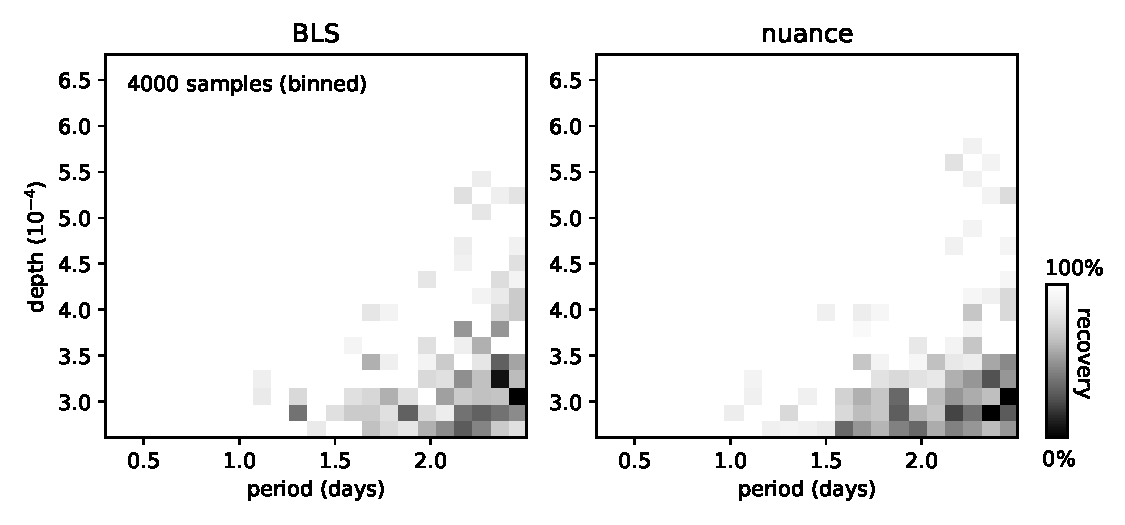
\includegraphics[width=\linewidth]{../workflows/control_test_bls/figures/control_test.pdf}
        \caption{Binned statistics of the injection-recovery of 4000 transit signals in a flat light curve with only white noise using BLS and \nuancecode{}. The color scale indicates the recovery of transits in the corresponding (period, depth) parameter space, white for a full recovery and black for no detection.}
        \label{fig:control}
    \end{centering}
\end{figure}

These results demonstrate the qualitative match between the detection capabilities of \textsf{nuance} and BLS on light curves with no correlated noise. Explaining the subtle differences observed between the two methods when only white noise is present is beyond the scope of this paper, and we will assume that any differences observed in the following sections are due to the different treatments of correlated noise.

\newpage
\section{Performances}\label{results}
\subsection{Comparison with \texttt{biweight+BLS} on simulated light curves}\label{simu}
\autoref{fig:snr_detrend} shows that \textsf{nuance}'s full-fledged modeling capabilities may not always be necessary and may only be beneficial for certain noise characteristics, relative to the searched transit parameters. Here, we evaluate the performance of \textsf{nuance} in the relative parameter space $(\tau, \delta)$ described in \autoref{eq:relative_params} and see when its specific treatment of correlated noise in the transit search becomes necessary.\\\\
We compare \textsf{nuance} to the approach that involves removing stellar variability from light curves before performing the search on a detrended dataset. Similarly to \autoref{detrending_effect}, an optimal bi-weight filter implemented in the \textsf{wõtan} Python package\footlink{https://github.com/hippke/wotan} is used with a window size three times that of the injected transit duration. A transit search on the detrended light curve is then performed using the BLS algorithm, like in \autoref{control} using the \textsf{astropy} \textsf{BoxLeastSquares} implementation\footlink{https://docs.astropy.org/en/stable/api/astropy.timeseries.BoxLeastSquares.html}; a strategy commonly used in the literature that we denote \texttt{biweight+BLS}. In what follows, the transit detection criteria are the same as the ones used in \autoref{control}, i.e. that a transit is considered recovered if the absolute difference between the injected and recovered period is less than 0.01 days, including periods found at half or twice the injected ones (aliases) and ignoring the value of the recovered transit epoch.

\subsubsection*{Dataset}\label{sim_dataset}
The dataset consists in 4000 light curves simulated using the model fully described in \autoref{signals_simulations}. We simulate a common periodic transit added to all light curves, of period $P=1.1$ days, epoch $T_0=0.2$ days, duration $D=0.04$ days and depth $\Delta=1\%$. Each light curve consists in a 4 days observation with an exposure time of 2 minutes, leading to $N=2880$ data points with a normal error of $0.1\%$. As in \autoref{control}, only box-shaped transits are injected, using the model from \cite{protopapas} with $c=500$ (cf.\;\autoref{app_proto}).\\\\
For a given pair of $(\tau, \delta)$, we simulate stellar variability using a GP with an SHO kernel of hyperparameters defined by \autoref{eq:relative_params} (except for $Q$, described below), computed with respect to the injected transit parameters $D$ and $\Delta$. The same kernel is used for the search with \textsf{nuance}, an optimal choice on equal footing with the optimal $3\times D$ window size of the bi-weight filter employed in the \wtls{} search.
%  While this kernel is optimal, a comprehensive discussion on the use of non-optimal kernels is discussed in . 
 4000 pairs of $(\tau, \delta)$ are generated such that
\begin{equation*}
    \tau \sim \mathcal{U}(0.1, 10), \hspace{0.5cm} \delta \sim \mathcal{U}(0.1, 25) \hspace{0.5cm}\text{and}\hspace{0.5cm} Q \sim \mathcal{U}(10, 100)
\end{equation*}
where $\mathcal{U}(a, b)$ denotes a uniform distribution of lower bound $a$ and upper bound $b$.

\subsubsection*{Results}
The results of this injection-recovery procedure are shown in \autoref{fig:simu} and highlight particularly well the benefit of \textsf{nuance} against the \wtls{} strategy on transits with relatively large depth compared to the stellar variability amplitude, and a relatively large duration compared to the stellar variability period. This empirical statement only concerns light curves with a given amount of white noise, and may vary depending on the length of the observing window or the number of transits. For this reason, quantifying for which values of $(\tau, \delta)$ \textsf{nuance} outperforms \wtls{} would only apply to this specific but representative example. However, we verify that our conclusions remain qualitatively valid for various simulation setups.
\begin{figure}[H]
    \begin{centering}
        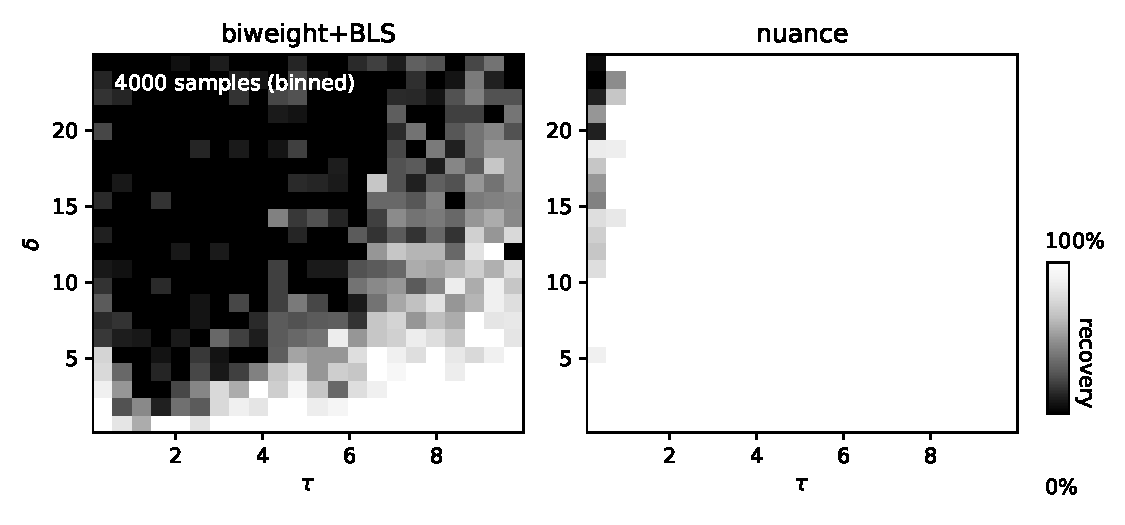
\includegraphics[width=\linewidth]{../workflows/synthetic-injection-recovery/figures/synthetic_ir.pdf}
        \caption{Injection-recovery results on 4000 simulated light curves described in \autoref{sim_dataset}. The color scale represents the fraction of recovered transits, white if all injected transits are recovered in a given portion of the $(\tau, \delta)$ parameter space, black if none are recovered.}
        \label{fig:simu}
    \end{centering}
\end{figure}

\noindent This injection-recovery is done in a particularly optimal setup, on light curves not all physically realistic and using an optimal GP kernel, hence demonstrating the performance of \textsf{nuance} only on a purely experimental basis. In the next section, we perform transits injection-recovery on real space-based light curves.

\newpage
\subsection{Comparison with various techniques on rapidly-rotating M dwarfs TESS light curves}\label{real}

% In order to validate 

% The parameter space ($\tau$, $\delta$) introduced in \autoref{detrending_effect} is very convenient from a signal processing point of view, but lacks physical reality. Very low values of $\tau$ and $\delta$ often translate into non-physical exoplanets properties as well as unrealistic stellar variability, with a strong dependence on the host star properties. \\\\
% In order to assess the performance of \textsf{nuance} on real light curves, its transit recovery capabilities are rather evaluated in the planetary (period, radius) parameter space, more often encountered in the literature (e.g. Figure 12 of \citealt{Delrez2022}). In what follows, transits described by the simple model of \cite{protopapas} (see \autoref{app_proto}) are 

In order to assess the performance of \nuance{} on real datasets, we inject and recover transits into light curves from the Transiting Exoplanet Survey Satellite (TESS, \citealt{tess}). The goal of this transit injection-recovery is to compare \nuance{} to other transit search strategies, and to understand the light curves characteristics for which it becomes beneficial.\\\\
We focus this proof of concept on light curves from a list of 438 M-dwarfs found to have detectable rotation signals with periods lower than one day \citep{Ramsay2020}, which lead to a parameter space justifying the use of \nuance{}. For each of the studied target, transits are injected and recovered in the TESS 2 min cadence SPOC Simple Aperture Photometry and Pre-search Data Conditioning light curves (PDCSAP, \citealt{spoc}) of a single sector (the first being observed for each target) spanning on average 10 days.\\\\
In this injection-recovery tests, \nuance{} is compared to other transit search strategies employing the BLS algorithm, for each of them after detrending the light curves with a different technique:
\begin{itemize}
    \item \texttt{bspline+BLS} employs a B-spline\footlink{https://docs.scipy.org/doc/scipy/reference/generated/scipy.interpolate.BSpline.html} for detrending, fitted using the \textsf{scipy.interpolate.splrep} function\footlink{https://docs.scipy.org/doc/scipy/reference/generated/scipy.interpolate.splrep.html}, followed by a search with the BLS algorithm.
    \item \texttt{biweight+BLS} employs an optimal bi-weight filter implemented in the \textsf{wõtan} Python package \citep{wotan} with an optimal window size of $3\times D$ (i.e.\, three times the transit duration), followed by a search with the BLS algorithm.
    \item \texttt{harmonics+BLS} employs a linear harmonic detrending, where the light curve is modeled as a Fourier series including four harmonics of the stellar rotation period found by \cite{Ramsay2020}, with coefficients found through ordinary least square. This detrending is followed by a search with the BLS algorithm.
    \item \texttt{iterative+BLS} iteratively detrends the light curve with a sinusoidal signal fitted to the data, each time using the dominant period of the residuals found using a lomb-scargle periodogram (5 iterations). This detrending is followed by a search with the BLS algorithm.\\\\
\end{itemize}


\subsubsection*{Light curve cleaning and transits injection}

As some of the techniques compare to \nuance{} can be affected by gaps in the data, we only use continuous measurements from half a TESS sector. We assume that all methods (including \nuance{}) are based on an incomplete model of the data that do not account for stellar flares. For this reason, the light curve of each target is cleaned using an iterative sigma clipping approach. For each iteration, points 3 times above the standard deviation of the full light curve (previously subtracted by its median) are identified. Then, the 30 adjacent points on each side of the found outliers are masked. This way, large flare signals and their expected ingress and egress are masked, using a total of 3 iterations. At each iteration, the GP kernel hyperparameters are re-optimized. As PDCSAP light curves often start with a ramp-like signal, the first 300 points (as well as the last 300 points) of each continuous observation are masked. Finally, each light curve is normalized by its median value. Such a cleaned light curve is shown in \autoref{fig:cleaned}. We note that the gaps left after sigma clipping may be problematic for some of the detrending techniques (such as \texttt{bspline+BLS}). However, adopting this flare cleaning step and analyzing light curves with few small gaps is a practice commonly found in the literature.
\begin{figure}[H]
    \centering
    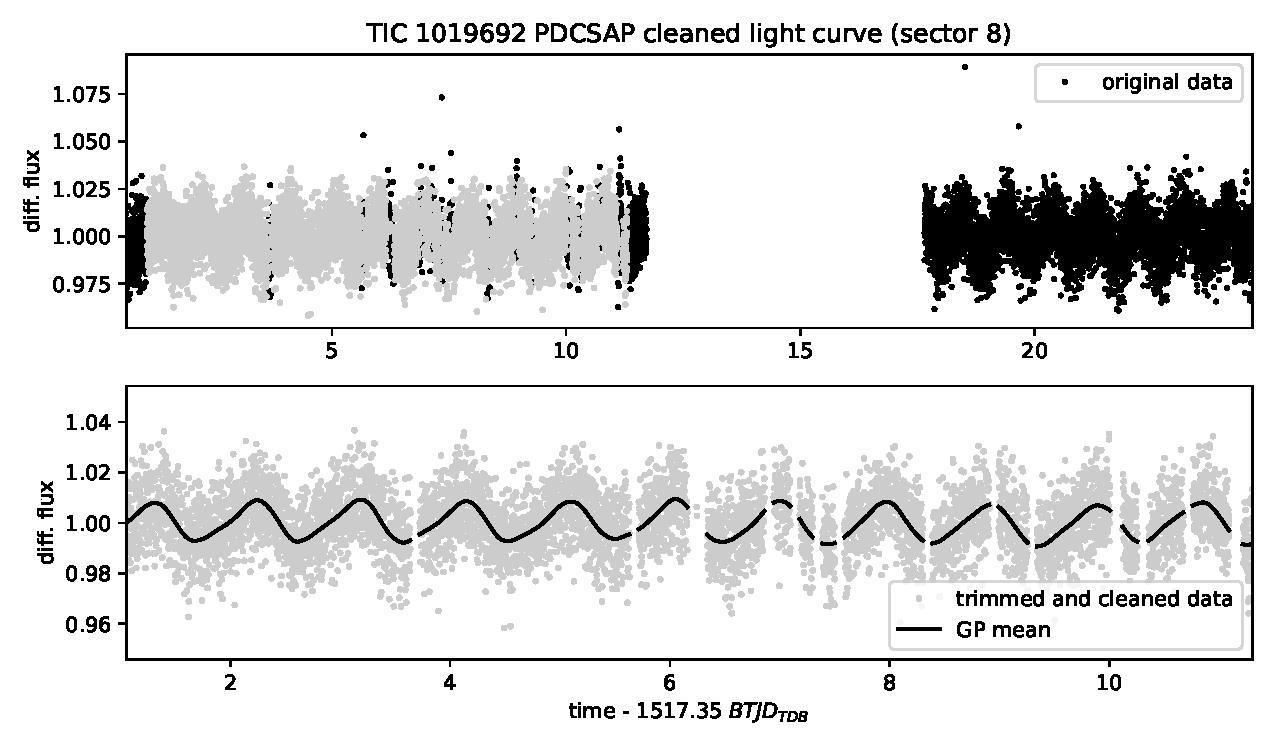
\includegraphics[width=\linewidth]{../workflows/tess_injection_recovery/figures/cleaned/1019692.pdf}
    \caption{Trimmed and cleaned single-sector light curve of the target TIC 1019692. Top plot shows how much of the data is truncated and sigma clipped, resulting in a quasi-continuous light curve shown in the bottom plot. On this bottom plot, the black line corresponds to the mean of the GP model (with hyperparameters optimized here on the cleaned light curve).}
    \label{fig:cleaned}
\end{figure}
For each light curve, transits of planets with 10 different orbital periods combined with 10 planetary radii are individually considered, for a total of 100 periodic transits injection-recovery per target. Orbital periods $P$ are sampled on a regular grid between 0.4 and 5 days, and planetary radii $R_p$ are sampled on a regular grid designed to yield a minimum transit SNR of 2 and a maximum of 30. Using \autoref{eq:snr} with $\sigma_r = 0$, the planetary radius leading to a transit with a desired SNR $s$ is given by
\begin{equation*}
    R_p = R_{\star}\,n^{-\frac{1}{4}} \sqrt{\sigma s}\ %\sqrt[\leftroot{0}\uproot{2}4]{n}}. 
\end{equation*}
with $\sigma$ equal to the mean uncertainty estimated by the SPOC pipeline, $R_\star$ the radius of the star reported by \cite{Ramsay2020} and $n$ the number of points in transit computed using a transit duration assuming a circular orbit.

\subsubsection*{Stellar variability kernel}\label{rotation_kernel}
One of the particularity of \nuance{} is to model a light curve as a GP. To model these TESS light curves, we employ a mixture of two SHO kernels of period $P_\star$ and $P_\star/2$ (with $P_\star$ the rotation period of the star), a model representative of a wide range of stochastic variability in stellar time series\footlink{https://celerite2.readthedocs.io/en/latest/api/python}. In order to account for additional corelated noises, we complement this kernel with a short and a long-timescale exponential term, so that the full kernel can be expressed as
\begin{equation*}
    k = k_1 + k_2 + k_3 + k_4
\end{equation*}
with
\begin{itemize}
    \item $k_1$ a SHO kernel with hyperparameters \begin{equation*}
        Q_1 = 1/2 + Q_0 + \delta Q\,, \hspace{0.5cm}
        \omega_1 = \frac{4\,\pi\,Q_1}{P\,\sqrt{4\,Q_1^2 - 1}} \hspace{0.5cm} \text{and} \hspace{0.5cm}
        S_1 = \frac{\sigma^2}{(1 + f)\,\omega_1\,Q_1}.
    \end{equation*}
    \item $k_2$ a SHO kernel with hyperparameters \begin{equation*}\begin{gathered}
        Q_2 = 1/2 + Q_0\,, \hspace{0.5cm}
        \omega_2 = 2 \omega_1 \hspace{0.5cm} \text{and} \hspace{0.5cm}
        S_2 = \frac{f\,\sigma^2}{(1 + f)\,\omega_2\,Q_2},
    \end{gathered}\end{equation*}
\end{itemize}
where $Q_0$ is the quality factor for the secondary oscillation, $\delta Q$ is the difference between the quality factors of the first and the second modes, $f$ is the fractional amplitude of the secondary mode compared to the primary and $\sigma$ is the standard deviation of the process. The kernels $k_3$ and $k_4$ are expressed as 
\begin{equation*}
        k(t, t')=\sigma^2\,\exp\left(-\frac{\vert t - t' \vert}{\ell}\right),
\end{equation*}
with $\ell$ and $\sigma$ the scale and standard deviation of the process. These are meant to model short and long-timescale non-periodic correlated noise. In total, the rotation kernel $k$ has 8 hyperparameters.\\\\

The hyperparameters of this kernel are optimized on trimmed and cleaned light curves containing the injected transits, using the \textsf{scipy.optimize.minimize}\footlink{https://jax.readthedocs.io/en/latest/_autosummary/jax.scipy.optimize.minimize.html} wrapper provided by the \textsf{jaxopt} Python package, and taking advantage of the \textsf{JAX} implementation of \textsf{tinygp}. As correlated noise is expected to affect the light curve uncertainty estimates performed by SPOC, the diagonal of the full covariance matrix of the data (i.e.\,their uncertainty, assuming homoscedasticity) is held free, increasing the number of optimized parameters to 9. The optimization is performed using the \textsf{BFGS} algorithm \citep{Fletcher1987}, minimizing the negative log-likelihood of the data as expressed in \autoref{eq:linear_search_ll} (without transit), i.e.\,accounting for a linear systematic model of the data in addition of stellar variability. For simplicity, and to adopt a uniform treatment for all target light curves, a design matrix $\bm{X}$ with a single constant column is adopted, such that the systematic model only consists in a single parameter corresponding to the mean value of the differential flux (expected to be close to 1) solved linearly. Our motivations to choose this very simplistic baseline, despite the capability of \nuancemethod{} to account for more complex linear models, is discussed in \autoref{systematics}.

\subsubsection*{Search parameters and transit detection criteria}
For all techniques, we only search for transits with a duration fixed to the known duration of the injected transits. This is mainly done for computational efficiency and allows for a narrower comparison between \nuancemethod{} and all BLS-based techniques. Finally, the search is done over 4000 trial periods linearly sampled from 0.3 to 6 days. A realistic transit search on a wider parameter space (e.g. multiple trial durations) is discussed in the next section.\\\\
Like in previous sections, we consider the detection of period aliases and ignore the match between the injected and recovered transit epochs (although we visually vet that the found epochs were consistent with the ones injected for cases where the planet was detected). We consider a transit detectable if its original SNR is greater than 6. Hence we define \textit{true positives} has detectable transits recovered with the correct period (or an alias) and a measured SNR greater or equal to 6, and \textit{false positives} as non-detectable transits recovered with a measured SNR greater or equal to 6.\\\\As we noticed that few methods were still affected by the remaining stellar variability after detrending, we remove from the grid of trial periods all periods close to the stellar rotation period and its aliases. In practice this is done by removing all periods $P$ such that $dP = \frac{P}{P_*}$ is less than 2\% from an integer value, i.e. $\vert  dP - \lceil dP \rceil \vert < 0.02$.

\newpage
\subsubsection*{Results}
An example of the transit injection-recovery and its result is shown in \autoref{1019692} for the target TIC 1019692. \autoref{fig:allsearch} shows the global results of the injection-recovery for all targets, while \autoref{fig:allsearch_relative} shows the true and false positives plotted against the relative parameters $\tau$ and $\delta$ (defined in \autoref{eq:relative_params}). Compared to other methods, we find that \texttt{nuance} leads to the highest number of true positives, with a successful detection of 76\% of the 7008 detectable transits and the lowest number of false negatives (\autoref{fig:allsearch}).
\begin{figure}[H]
    \begin{centering}
        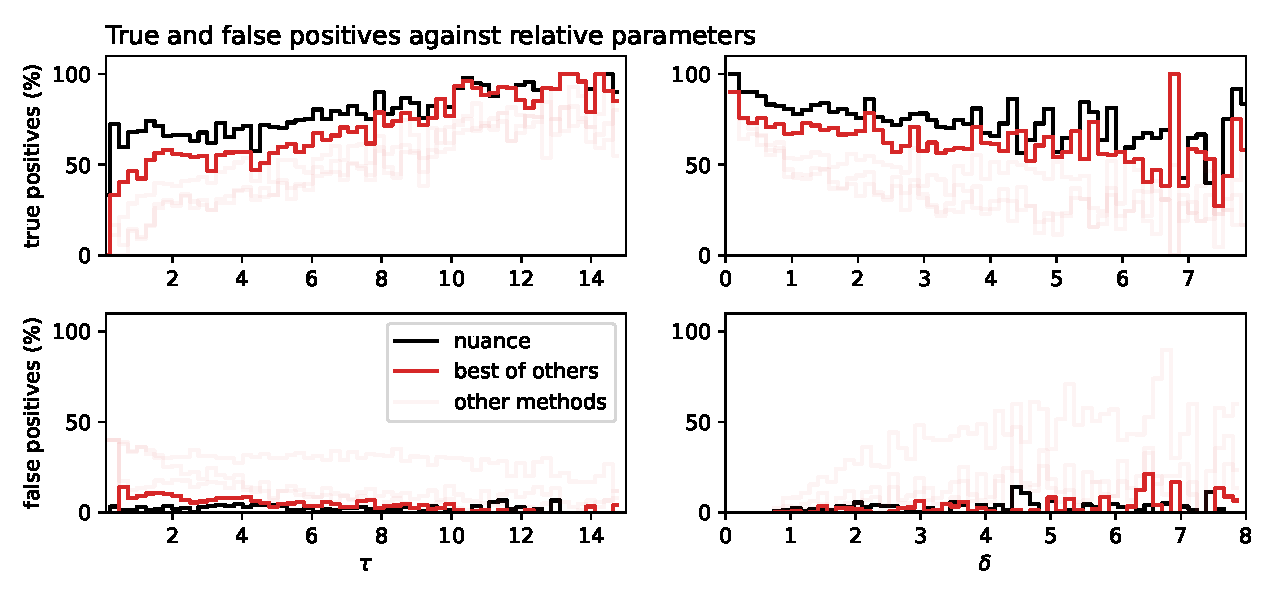
\includegraphics[width=\linewidth]{../workflows/tess_injection_recovery/figures/true_false_positives.pdf}
        \caption{Rate of true and false positives of \nuance{} compared to other methods, as a function of the relative parameters $\tau$ and $\delta$. The solid red line corresponds to the maximum of true positives among all methods on the top panel, and the minimum of false positives on the bottom panel.}
        \label{fig:allsearch_relative}
    \end{centering}
\end{figure}
\begin{figure}[H]
    \begin{centering}
        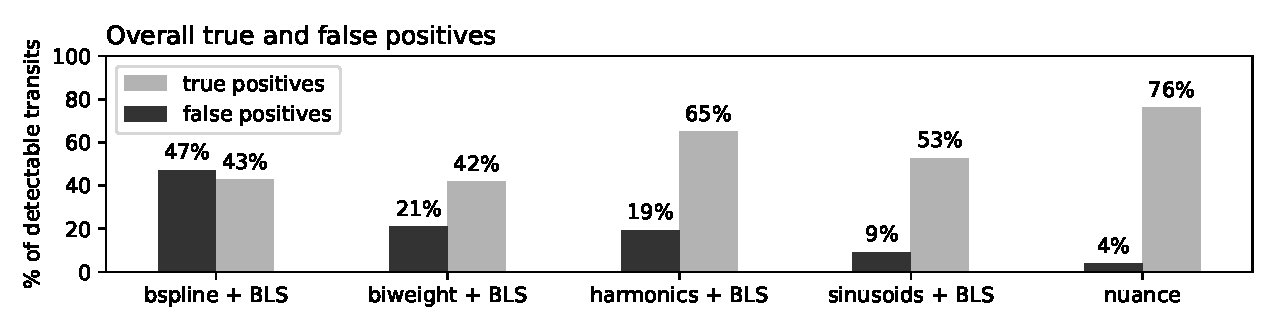
\includegraphics[width=\linewidth]{../workflows/tess_injection_recovery/figures/true_and_false_positives_bars.pdf}
        \caption{Rate of true and false positives for all methods as a fraction of detectable transit signals.}
        \label{fig:allsearch}
    \end{centering}
\end{figure}
While the performances of other methods highly depend on the characteristics of the variability, \nuance{} leads to the highest number of true positives in 79\% of cases, and the lowest number of false positives in 72\% of cases (\autoref{fig:allsearch_relative}). When considering both true and false positives simultaneously, \nuance{} can be considered the best technique in only 55\% of cases. However, \textbf{when considering transits with a relative timescale $\tau < 5$ (transits that justified the development of this algorithm), \nuancemethod{} is the best technique in 94\% of cases, leading to both the highest number of true positives and the lowest number of false positives}.

\subsection{Comparison for a multi-sector TESS candidate: TOI-540}\label{toi540}

In order to further validate nuance on a realistic dataset, we focus this section on the multi-sector TESS light curves of TOI-540, and the search for its earth-like companion TOI-540 b \citep{TOI540}. We download the 2 minutes cadence SPOC PDCSAP light curves of TOI-540 observed in 5 sectors (4, 5, 6, 31 and 32). Like in the previous section, we use a Lomb-Scargle periodogram and identify the 0.72 days rotation period of the star, that we use as an initial value to optimize the kernel described in \autoref{rotation_kernel} on each sector independently. Here again, we employ an upper-sigma-clipping to mask flares out of the data. The resulting light curve for sector 4 and its mean model are shown in \autoref{fig:toi540_clean}.
\begin{figure}[H]
    \begin{centering}
        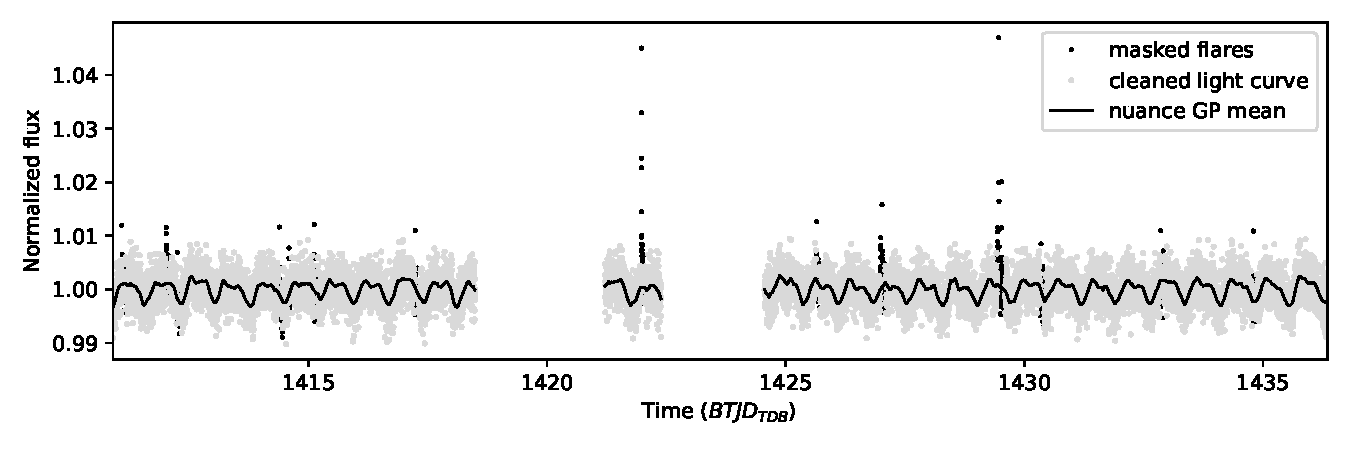
\includegraphics[width=\linewidth]{../workflows/comparison_toi/figures/TOI 540/4.pdf}
        \caption{Sector 4 light curve of TOI 540. The cleaned signal (gray points) has been masked for flares (black points), and the black line corresponds to the mean of the GP model.}
        \label{fig:toi540_clean}
    \end{centering}
\end{figure}

For each sector, we perform the linear search of nuance on the cleaned light curve, using the original times as the trial epochs and 10 trial transit durations linearly sampled from 15 minutes to 1.5 hours. We then perform the periodic search on all sectors combined, using a concatenation of all linear searches. By adopting this by-sector GP modeling of the light-curve, the linear search of \nuance{} scales linearly with the number of sectors being processed. This approach is adopted for efficiency but also to encapsulate the changing properties of stellar variability from one sector to another, often separated by year-long gaps. The periodic search is done on 20 000 trial periods ranging from 0.5 to 10 days. This search, using \nuancecode{}, is compared to the more traditional approach that consists in detrending each sector with a bi-weight filter and then search for transits with the BLS algorithm (denoted \texttt{biweight+BLS} and described in \autoref{real}) on all sectors combined. Since we don't know the transit duration a-priori, we perform the detrending and BLS search using 15 filtering window sizes sampled from 30 minutes to 5 hours, and retain the search that leads to the highest transit SNR peak in the periodogram (as done e.g.\;in the SHERLOCK transit search pipeline described in \citealt{Pozuelos2020}). The results of this comparison are shown in \autoref{fig:toi540_periodograms}.
\begin{figure}[H]
    \begin{centering}
        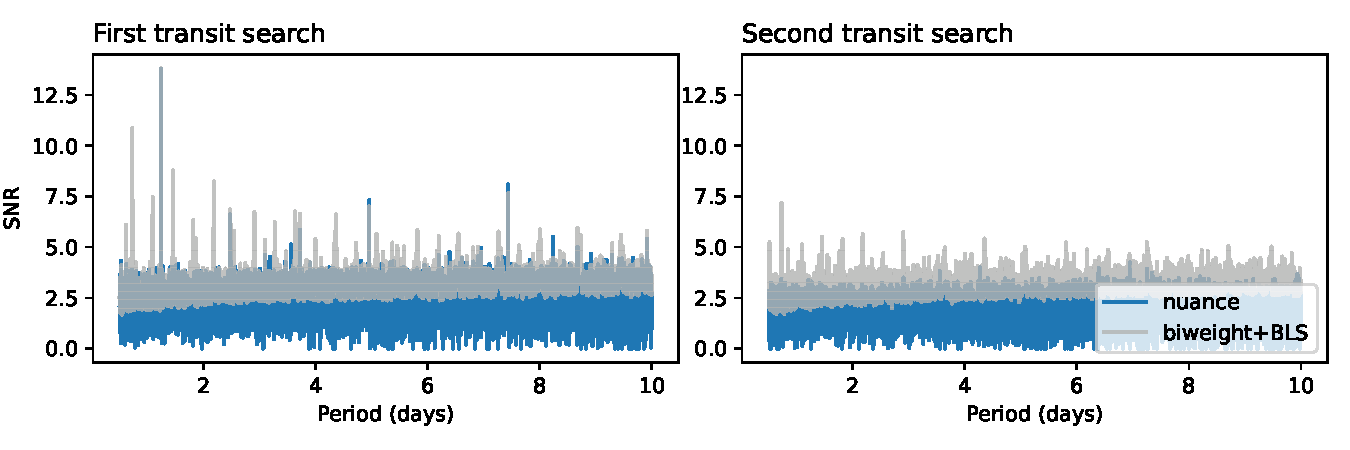
\includegraphics[width=\linewidth]{../workflows/comparison_toi/figures/TOI 540/periodograms.pdf} 
        \caption{Transit search SNR periodograms of TOI-540 using \texttt{biweight+BLS} and \nuance{}. After a first periodic search (left panel), the epochs corresponding to the maximum-SNR transit are masked before the second search is performed (right panel).}
        \label{fig:toi540_periodograms}
    \end{centering}
\end{figure}
After a first periodic search, trial epochs in windows of widths $2\times D$ centered on the detected periodic transits are masked. In practice, this is done by masking the linear search products $\set{\ln\mathcal{L}_{i,j}}_{i, j}$, $\set{\Delta_{i,j}}_{i, j}$ and $\set{\sigma_{i,j}}_{i, j}$ (defined in \autoref{linear_search}).\\\\
As seen in \autoref{fig:toi540_periodograms}, the SNR periodogram using \texttt{biweight+BLS} and \texttt{nuance} are very similar, with the known transiting exoplanet TOI-540 b detected with an orbital period P = 1.24 days. This is well expected as the relative parameter $\tau$ equal 13 for TOI-540 b \footnote{using \autoref{eq:relative_params} with the stellar rotation $P=0.72$ days and the known transit duration $D=29.5$ min of TOI-540 b \citep{TOI540}}, which lies outside the range where \nuancemethod{} is expected to be beneficial beneficial (see \autoref{fig:snr_detrend}). Nonetheless, the \nuance{} periodogram of TOI 540 features less spurious SNR peaks, largely due to the penalty naturally occurring when single transits with different depths are periodically combined. In the second search (right panel) of \autoref{fig:toi540_periodograms}, we also notice a higher number of peaks that would lead to false positive detections of transits in the \texttt{biweight+BLS} case. The proper treatment of correlated noise in \nuance{}, as observed in \autoref{real}, makes these peaks non-significant, avoiding a large number of false detections.\\\\
We note that finding a TESS candidate that displays characteristics for which \nuance{} is expected to be significantly beneficial proved to be very challenging during the writing of this paper, as transits with such characteristics are expected to be missed by current state-of-the-art techniques (see e.g.\;\autoref{fig:simu}). Nontheless, we verify that \nuancemethod{} is capable of finding a large number of already known transiting exoplanet candidates, in light curves featuring various forms of correlated noises, at least as efficiently as with commonly used techniques. We reserve the search for new transit signals to a follow-up publication.

\section{Discussion}\label{discussion}

In the previous section we demonstrated the capability of \nuance{} to search for synthetic or known transit signals, in simulated or real datasets. Here, we discuss the caveats of this algorithm, the advantages and limitations of the \nuancecode{} implementation, and future prospects for its extension.

\subsection{Processing time}

\noindent In \autoref{fig:blsvsnuance}, the processing time of \nuancecode{} linear and periodic search are recorded against the number of points in a simulated light curve, assuming a simple non-optimized GP with a squared exponential kernel. These are compared to the processing time of \texttt{biweight+BLS} (cf.\;\autoref{simu}) separated into the bi-weight filtering step and the BLS search.
\begin{figure}[H]
    \begin{centering}
        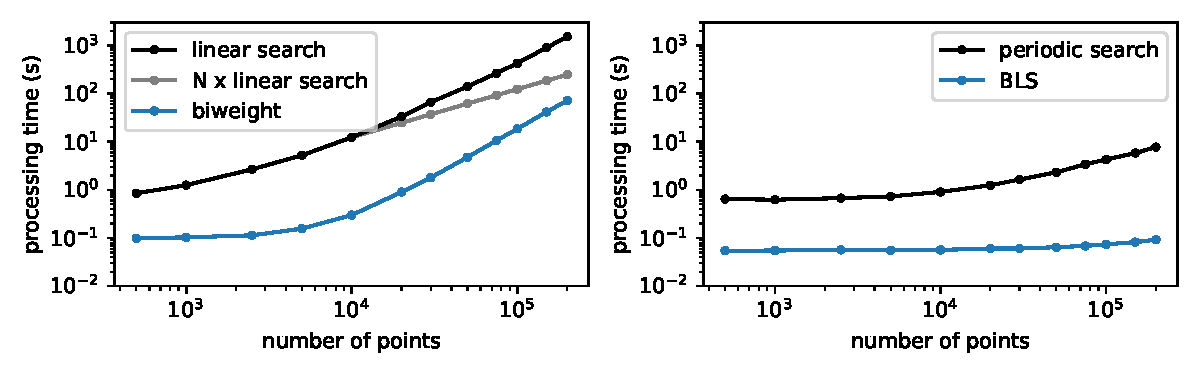
\includegraphics[width=\linewidth]{../workflows/benchmark/figures/nuance_vs_bls.pdf}
        \caption{Study of \textsf{nuance} (black line) processing time against \texttt{biweight+BLS} (cf.\;\autoref{simu}, blue line). The gray curve shows the performance of \textsf{nuance} \textit{linear search} when applied to chunks of 10 000 points continuous observations, instead of considering these observations all together. This study is performed on the 12 cores of an Apple M2 Max chip, exploiting the parallelization offered by our implementation. While not being shown, we verify that both the BLS algorithm and \nuancemethod{} processing times scale linearly with the number of probed transit durations and orbital periods.}
        \label{fig:blsvsnuance}
    \end{centering}
\end{figure}

As see in \autoref{fig:blsvsnuance}, most of the computational costs of \nuancecode{} and the \texttt{biweight+BLS} method in this particular example come from the linear search and the bi-weight filtering step. This is not always true and depends on the size of the trial durations and periods grids. One advantage of \nuancemethod{} is that the linear search can be performed separately on different continuous observations, and then combined in the periodic search. Hence, if searching for transits in separate observations with approximately similar durations, such as different TESS sectors or different ground-based nightly observations, the computational cost of \nuancecode{} grows linearly with the number of observations (see grey line in \autoref{fig:blsvsnuance}). Nonetheless, considering a variety of other detrending algorithms, \textbf{\nuancecode{} is expected to perform about one order of magnitude slower than more conventional techniques associated with BLS}. The second advantage of \nuancecode{} is its \textsf{JAX} implementation, allowing the linear search to be run in parallel. As a reference, searching for TOI-540 b transits with nuance (\autoref{toi540}), on the 12 cores of an Apple M2 Max chip, took 5 minutes 35 seconds in total, 1 minute 50 seconds for the 5 sectors linear searches (around 22 seconds each), and 3 minutes 45 seconds for the combined periodic search. In comparison, the brute force search with \texttt{biweight+BLS}, consisting in trying 15 bi-weight windows, took a total of 1 minute 49 seconds (about only 7 seconds each).\\\\
% As the periodic search is expected to be improved by lower lever optimizations (using a compiled language), we reserve its benchmark for a future work. Thanks to its \textsf{JAX} implementation, we also note the possibility of running \nuancecode{} on GPUs, which is out of the scope of the present comparison.\\\\
Because of its computational cost, \nuancecode{} must not be employed in the general case, but rather adopted when light curves contain correlated noise with specific characteristics. If employing a bi-weight filter for detrending, these characteristics correspond to the ones discussed in \autoref{issues}. But as these strongly depend on the type of detrending technique employed, we do not provide general guidelines as when \nuancemethod{} should be preferred over a specific detrending technique. To aid users in making an informed choice of algorithm, extensive benchmarks and guidelines are reserved to future developments and will be progressively shared on \nuancecode{}'s online documentation\footlink{https://nuance.readthedocs.io/en/latest/}.

\subsection{Systematics modeling}\label{systematics}
Throughout the paper, a single column design matrix $\bm{X}$, corresponding to the mean differential flux (ideally unitary), was employed, hence assuming that the instrumental systematics signals were non-existent. In practice, \nuancemethod{} has been developed to linearly model systematic signals through more complex design matrices (as in \citealt{foreman2016}), in addition with its capability to model correlated noise while searching for transits. This feature is intentionally unexploited in the comparisons presented in \autoref{results}, as detrending light curves assuming a linear systematics model, such as PLD co-trending vectors \citep{pld}, is highly incomplete if applied on data while ignoring the presence of other astrophysical signals. Comparisons involving more complex design matrices would also be sensitive to the choice of linear components, and would have unwanted repercussions on their results.\\\\
As an illustration, the NEMESIS pipeline \citep{nemesis} starts processing the differential light curves by employing a linear systematics detrending using a least square fit of the data with a reduced PLD basis, before smoothing the signal from stellar variability using an approach similar to the one employed in the \texttt{biweight+BLS} approach (cf.\;\autoref{real}), hence detrending the systematics with an incomplete model that does not account for stellar variability. To account for stellar variability while fitting the linear systematics model to the data, a step further would be to use a GP, such as done in the EVEREST \citep{everest2} pipeline. However this would also involve some potential degradation of the transit signals (see e.g.\;\autoref{fig:issue2}), with an hardly distinguishable origin. For these reasons, and to keep our comparisons as targeted as possible, we do not compare commonly used systematics detrending approaches and decided to focus our comparisons solely on stellar variability detrending techniques (although these two aspects often overlap in the literature).\\\\
Although not being demonstrated here, modeling systematics signals while searching for transits on data acquired sparsly is extremely promising for the search of transiting exoplanets in ground-based data, that usually suffer from daily interruptions. In this respect, we note the similarity of our \textit{linear search} (cf\;\autoref{linear_search}) to the one presented in \citealt{Berta2012}, that focused on the detection of single eclipses in the MEarth light curves \citep{Irwin2009}. Similarly, \textbf{\nuancemethod{} would highly benefit the search for transiting exoplanets around M-dwarf type stars}, such as the ones observed by the SPECULOOS survey \citep{speculoos} whose monitoring suffers from both increased red noise (due to atmospheric and instrumental thermal effects discussed e.g.\;in \citealt{Berta2012} and  \citealt{Pedersen2023}) and enhanced stellar variability \citep{Murray2020}. We reserve this promising application to a future study.

\subsection{The choice of kernel}
While not being discussed in our study, \textbf{the efficiency of \nuancemethod{} to detect transits in correlated noise is highly dependant on the design of its GP kernel}. In the ensemble comparison of \autoref{real}, the goal was to choose a kernel and an optimization strategy suited to most of the studied light curves, leading to few outliers in the results that were indicative of a badly designed and/or optimized kernel. An alternative, recommended for more realistic blind searches, is to perform model comparison on well selected kernels, and to adapt the optimization strategy to each dataset.\\\\
When using \nuancecode{} on TESS light curves for example, it must be noted that the observed light curve variability might originate from a contaminated photometric aperture, so that a physically-interpretable GP kernel representing a single star activity is not necessarily appropriate. On the other hand, a single squared exponential GP kernel might also be sufficient for some applications.

\subsection{Prospects}
The present implementation of \nuancemethod{} has the potential to be extended to be used beyond the search of periodic transits. Here are ideas of possible use and extensions, from the most straightforward to the most ambitious:
\begin{enumerate}
    \item In order to compare \nuancecode{} to BLS-based methods, we injected and retrieved only box-shaped transits. However, similarly to the Transit-Least-Square algorithm from \cite{tls}, \textbf{limb-darkened transits can serve as base model} in the linear search and are expected to improve the transit search in the same way TLS provided an improvement over BLS.
    \item The linear search of \nuancemethod{} is a single-event detection algorithm that can be used to search for single transit events, but also \textbf{detect transiting exocomets and flares}, by simply adapting the base astrophysical model in the last colum of the design matrix $\bf{X}$. While not being tested and benchmarked, the \nuancecode{} implementation already integrates this feature (make a tutorial!).
    \item During the periodic search, no prior about the transit duration related to the orbital period of the planet was used. This was done in order to allow the detection of grazing transiting exoplanets that would produce shorter timescale transits compared to what is expected from a circular orbit. However, adding such prior, \textbf{using the distribution of known exoplanets eccentricities}, might produce less spurious periodogram peaks and be very beneficial for the automatic search of transits in large datasets. Another idea, similar to the one employed in \cite{foreman2016}, is to leverage \textbf{model comparison in order to reject single transits that are better described by the GP model alone}. Both ideas come at no cost given our modeling approach.
    \item Finally, the formalism of \nuancemethod{} could be adapted and used to \textbf{search for exoplanets featuring transit time variations (TTV)}. Indeed, this application only requires a modification of the periodic search, as maximum likelihood peaks close to linearly predicted transit epochs may be considered. This could be done either with a special nearest-neighbor algorithm or with a convolution of the computed likelihood grid with a Gaussian kernel. To maximize efficiency and interpretability, we would recommend these approaches to be explored analytically, rather than using a data-driven treatment of the linear search products.
\end{enumerate}


\section{Conclusion}
This paper presents \nuancemethod{}, an algorithm designed to detect planetary transits in light curves featuring correlated noise in the form of instrumental signals and stellar variability. In this context, a conventional approach involves detrending a light curve before searching for transits using a Box-Least-Square algorithm. However, we show that the incomplete modeling of a light curve for its detrending, one that ignores the presence of transits, degrades their signal-to-noise-ratio down to the point of not being detectable. Adopting a widely used detrending stratgey, we explore the extend of this degradation on simulated light curves, and its dependance on the stellar variability characteristics.\\\\
The effectiveness of \nuancemethod{} is tested using a synthetic dataset and further validated on real TESS light curves of 438 M dwarfs. These injection-recovery tests reveal that \nuancemethod{} consistently outperforms conventional transit search techniques, especially for transits with duration exceeding one-fifth of the stellar variability timescale. In these cases, \nuancemethod{} not only identifies a higher number of true positive detections but also minimizes false positives, demonstrating its robustness and reliability.\\\\
To make \nuancemethod{} accessible for wider use, we make \nuancemethod{} publicly available through the \nuancecode{} open-source Python package. This package leverages the power of JAX, allowing for efficient computations and compatibility with distributed computing environments and GPU devices.\\\\
We acknowledge the limitations of \nuancemethod{} and its increased computational cost. In this regard, \nuancemethod{} should be used as an alternative to more traditional techniques only in the presence of substantial correlated noise. As guidelines for choosing \nuancemethod{} over other techniques are highly dependant on the type of detrending algorithm employed, we reserve this study to a future work.\\\\
Finally, we suggest future improvements and extensions of the algorithm, including its application for detecting single transits, exocomets, flares, and transit time variations (TTV), underscoring its versatility and potential for broader impact in astronomical research.
\\\\
\vfill{}
We would like to thank Julien De Wit, Prajwal Niraula and Francisco J. Pozuelos for meaningful discussions at the beginning of this project, Germain Garcia for his useful insights about numerical optimization, Michaël Gillon for his overall support, and the member of the Astronomical Data Group at the Center for Computational Astrophysics for many enriching discussions and feedback.x

\newpage
\appendix
\section{Light curves simulations}\label{signals_simulations}

In order to study the effect of correlated noise on transit search, this paper relies on transit light curve simulations including realistic effects of stellar variability and instrumental signals. The following describes how such signals are modeled.
\begin{figure}[H]
    \begin{centering}
        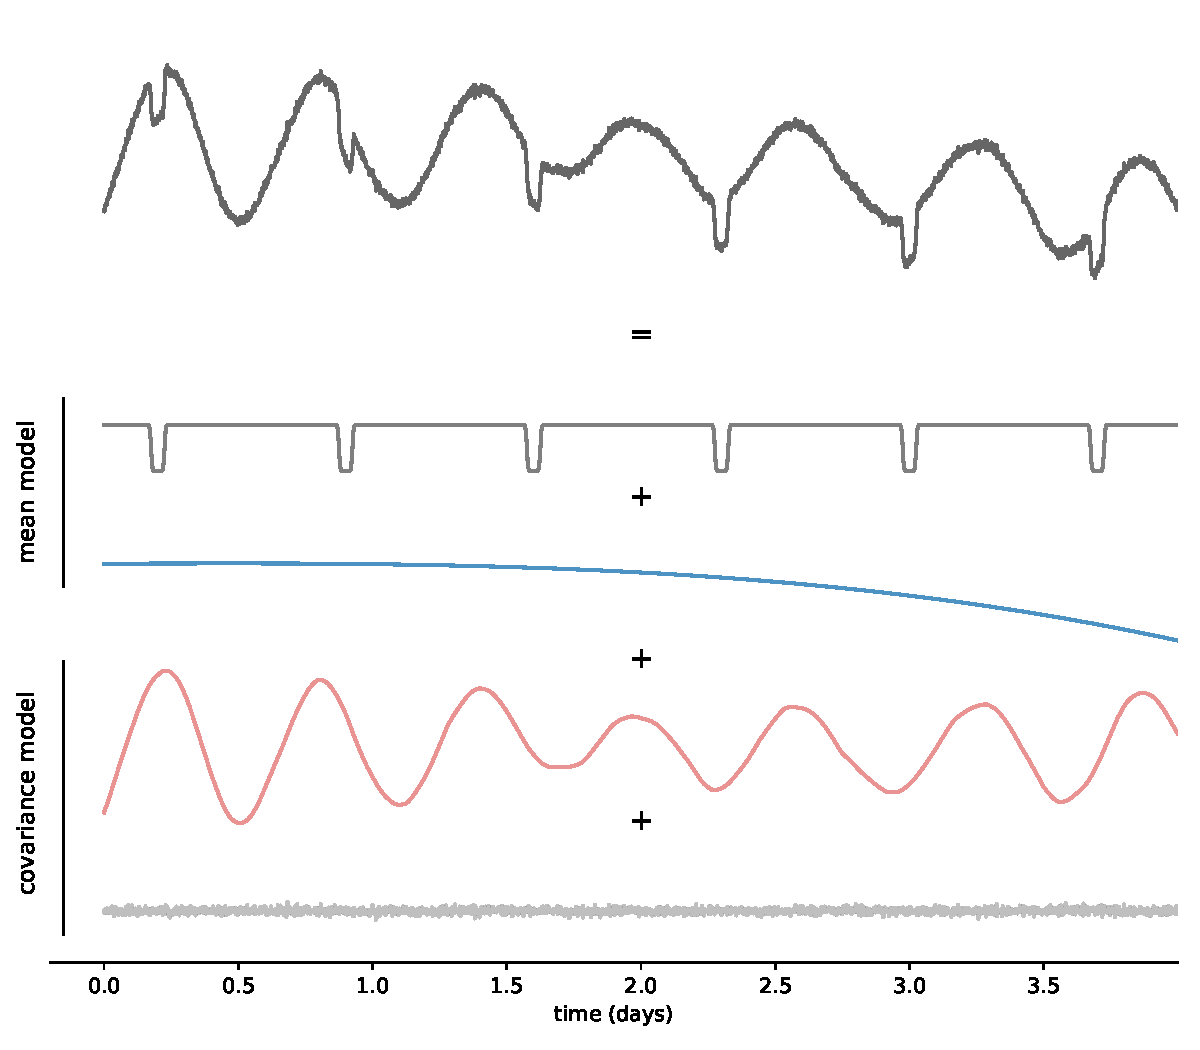
\includegraphics[width=\linewidth]{../workflows/principle/figures/principle_dataset_decomposed.pdf}
        \caption{Example dataset sampled at $N=2880$ times corresponding to an observation of 4 days with an exposure time of 2 minutes. The mean of this signal consists in a periodic transit signal of period $P=0.7$ days, duration $D=0.05$ days and depth of 2\% ($\mathcal{T}$ in gray) plus instrumental signals ($\mathcal{S}$ in blue). Correlated noise in the form of stellar variability is simulated by modeling the covariance matrix of the signal with a GP ($\mathcal{V}$ in red) including a diagonal variance of $0.001^2$ corresponding to white noise ($\epsilon$ in light grey). This simulated signal is not intended to be physically realistic.}
        \label{fig:app_principle_dataset}
    \end{centering}
\end{figure}
\noindent Let $f$ be the simulated flux of a star sampled and arranged in the vector $\bm{f}$ associated to the vector of times $\bm{t}$, such that
\begin{equation*}
    \bm{f} \sim \mathcal{N}(\bm{\mu}, \bm{C}),
\end{equation*}
i.e. that $\bm{f}$ is drawn from a GP of mean $\bm{\mu}$ and covariance matrix $\bm{C}$. In this equation, $\bm{\mu}$ is such that its $i$-th element is defined by  $\mu_i = \mathcal{T}(t_i) + \mathcal{S}(t_i)$ where $t_i$ is the $i$-th time of observation, $\mathcal{T}$ is a periodic transit function and $\mathcal{S}$ a function describing the instrumental part of the signal (both described below). The covariance matrix $\bm{C}$ is built such that $C_{i, j} = k(t_i, t_j)$ where $k$ is a covariance function (or \textit{kernel}) accounting for correlated noise in the form of stellar variability (with added white noise). An example of such signal is simulated and shown in \autoref{fig:app_principle_dataset}.

\subsection{Transit signal $\mathcal{T}$}\label{app_proto}
The periodic transit signal $\mathcal{T}$ is simulated using the simple model described in \cite{protopapas}, where a transit of period $P$, epoch $T_0$, duration $D$ and unitary depth observed at time $t$ is given by
\begin{equation}\label{eq:protopapas}
    \begin{gathered}
        \mathcal{T}_c(t, P, T_0, D) = \frac{1}{2}\tanh\left(c\left[\theta - \frac{1}{2}\right]\right) - \frac{1}{2}\tanh\left(c\left[\theta + \frac{1}{2}\right]\right), \\
        \text{with}\quad\theta = \frac{P}{\pi  D}\sin\left(\frac{\pi(t-T_0)}{P}\right),
    \end{gathered}
\end{equation}
where the dimensionless parameter $c$ controls the roundness of the transit depth ($c\gg1$ corresponding to a box-shaped transit as shown in \autoref{fig:protopapas}). This analytical model is fully empirical but easily differentiable.
\begin{figure}[H]
    \begin{centering}
        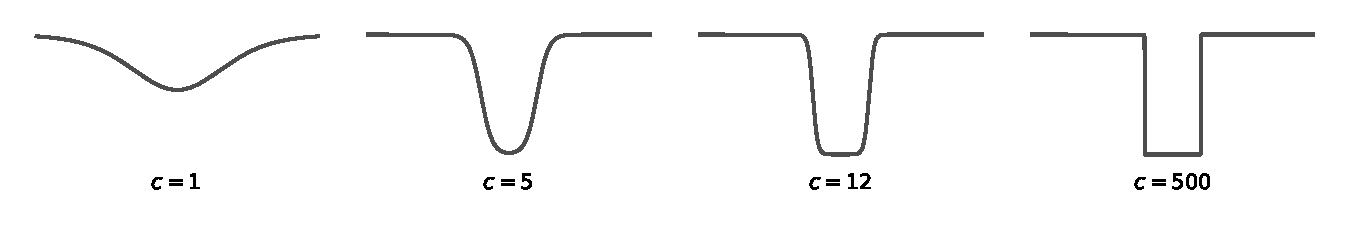
\includegraphics[width=\linewidth]{../workflows/principle/figures/protopapas.pdf}
        \caption{Simulations of a single transit signal (\autoref{eq:protopapas}) shown for different values of $c$.}
        \label{fig:protopapas}
    \end{centering}
\end{figure}
\noindent In this paper, unless specified, all transits are simulated with $c=12$, a value arbitrarily chosen that can be fined-tuned in real applications using the limb-darkening coefficients of a given star. The periodic transit signal $\mathcal{T}$ seen in \autoref{fig:app_principle_dataset} corresponds to $\mathcal{T} = 0.02 \times \mathcal{T}_{c=12}(\bm{t}, P=0.7, T_0=0.2, D=0.05)$, all parameters in unit of days.

\subsection{Instrumental signals $\mathcal{S}$}
Instrumental signals are simulated as a linear model of $M$ explanatory variables arranged in the $(N\times M)$ design matrix $\bm{X}$. Hence,
$$
    \mathcal{S} = \bm{X w},
$$
where the vector $\bm{w}$ contains the linear coefficients of the model. The simulated flux shown in \autoref{fig:app_principle_dataset} contains a linear model where the $M=4$ columns of the design matrix $\bm{X}$ are given by $\bm{X}_{i} = \bm{t}^i$ (i.e. $\bm{X}$ is the Vandermonde matrix order $3$ of time $t$) and $\bm{w} = [1.0\quad0.0005\quad\text{-}0.0002\quad\text{-}0.0005].$

\subsection{Stellar variability $\nu$}\label{app_gp}
As this chapter focuses on stellar variability and its effect on transit detection, We employ a simple physically-motivated GP kernel, describing stellar variability through the covariance of a stochastically-driven damped harmonic oscillator (SHO, \citealt{celerite, celerite2}) taking the form 
\begin{equation}
    \begin{gathered}
        k(\tau) = \sigma^2\,\exp\left(-\frac{\omega\,\tau}{2\,Q}\right)
        \left\{\begin{array}{ll}
            1 + \omega\,\tau & \mbox{for } Q = 1/2 \\
            \cosh(f\,\omega\,\tau/2\,Q) + \sinh(f\,\omega\,\tau/2\,Q)/f
                & \mbox{for } Q < 1/2 \\
            \cos(g\,\omega\,\tau/2\,Q) + \sin(g\,\omega\,\tau/2\,Q)/g
                & \mbox{for } Q > 1/2
        \end{array}\right. \\
        \text{where}\quad \tau = |t_i - t_j|\text{,}\quad f = \sqrt{1 - 4\,Q^2} \quad \text{and}\quad g = \sqrt{4\,Q^2 - 1}
    \end{gathered}
\end{equation}
where $Q$ is the quality factor of the oscillator, $\omega$ its pulsation and $\sigma$ the amplitude of the kernel function. GP computations in this paper use the implementation from \texttt{tinygp}\footnote{\href{https://github.com/dfm/tinygp}{https://github.com/dfm/tinygp}}, a Python package exposing the quasi-separable kernels from \cite{celerite2} and powered by \texttt{JAX}\footnote{\href{https://github.com/google/jax}{https://github.com/google/jax}}. The stellar variability signal in \autoref{fig:app_principle_dataset} has been sampled from a GP with an SHO kernel of parameters $\omega = \pi/6D$ (i.e. a period equal to 12 times the duration $D$ of the simulated transit), $Q=45$ and $\sigma=0.02$, the depth of the simulated transit. An extra term $\sigma_f^2=0.001^2$ is added to the diagonal of the covariance matrix, corresponding to the variance of the simulated measurement $f$ and leading to the white noise observed in \autoref{fig:app_principle_dataset}.

\section{Proof for the periodic search expression}\label{proof}

\newcommand{\sumTk}{i\neq k}
From the \textit{linear search} presented in \autoref{linear_search}, we retain and index by $k$ the parameters of the $K$ individual transits whose epochs $\{T_k\}_k$ are compatible with a periodic signal of period $P$ and epoch $T_0$. From the likelihoods of these transits (computed in \autoref{linear_search}), we want an expression for
\begin{equation*}
    p(\bm{f} \vert P, T_0 ,D, \Delta) = \prod_{k\in\mathbb{T}} p(\bm{f} \vert T_k, D, \Delta),
\end{equation*}
i.e., given a depth $D$, the likelihood of the data given a periodic transit signal of period $P$, epoch $T_0$ and a common depth $\Delta$. Since only $\{p(\bm{f} \vert T_k, D, \Delta_k)\}_{k}$ is known (i.e. transits with different depths), we decompose
\begin{equation}\label{eq:non_part_of_per}
    p(\bm{f} \vert T_k, D, \Delta) = \int p(\bm{f} \vert T_k, D, \tilde\Delta)p(\tilde\Delta | \Delta)\, d\tilde\Delta,
\end{equation}
where $p(\bm{f} \vert T_k, D, \tilde\Delta)$ is the probability of the $k$-th transit to have a depth $\tilde\Delta$ and $p(\tilde\Delta | \Delta)$ the probability to observe the depth $\tilde\Delta$ knowing the existence of a common depth $\Delta$. In other words, \autoref{eq:non_part_of_per} involves the likelihood of the non-periodic transit $k$ to be part of a periodic transit signal with a common depth $\Delta$.
\\\\
Since each depth $\Delta_k$ is found through generalized least square, each follow a normal distribution $\mathcal{N}(\Delta_k, \sigma_k^2)$, centered on $\Delta_k$ with variance $\sigma_k^2$ and an amplitude $\mathcal{L}_k$, leading to the likelihood function
\begin{equation*}
    p(\bm{f} \vert T_k, D, \tilde\Delta) = \mathcal{L}_k\exp \left(-\frac{(\tilde\Delta-\Delta_k)^2}{2\sigma_k^2}\right).
\end{equation*}
As for the common transit depth $\Delta$, it can be estimated through the joint probability of all other transit depths than $\Delta_k$, such that
\begin{equation*}
    \Delta \sim \prod_{\sumTk}^K \mathcal{N}(\Delta_i, \sigma_i^2),
\end{equation*}
with 
\begin{equation}\label{eq:params}
\frac{1}{\sigma^2} = \sum_{\sumTk}^K \frac{1}{\sigma_i^2} \hspace{0.5cm} \text{and} \hspace{0.5cm}
\Delta =\sigma^2 \sum_{\sumTk}^K {\frac{\Delta_i}{\sigma_i^2}}.
\end{equation}
Hence
\begin{equation*}
    p(\tilde\Delta | \Delta) = \frac{1}{\sqrt{2\pi\sigma^2}}\exp \left(-\frac{(\tilde\Delta-\Delta)^2}{2\sigma^2}\right).
\end{equation*}
We can now rewrite \autoref{eq:non_part_of_per} as
\begin{equation*}
    p(\bm{f} \vert T_k, D, \Delta) =  \frac{\mathcal{L}_k}{\sqrt{2\pi\sigma^2}} \int \exp\left(-\frac{(\tilde\Delta-\Delta_k)^2}{2\sigma_k^2}\right)\, \exp\left(-\frac{(\tilde\Delta-\Delta)^2}{2\sigma^2}\right)\, d\tilde\Delta.
\end{equation*}
The integral in this equation is a product of gaussian integrals that can be obtained analytically, leading to
\begin{equation*}
    p(\bm{f} \vert T_k, D, \Delta) = \mathcal{L}_k  \sqrt{\frac{\sigma_{k}^2}{\sigma^{2} + \sigma_{k}^{2}}} \exp\left(-\frac{1}{2}\frac{(\Delta_k-\Delta)^2}{\sigma_k^2 + \sigma^2}\right).
\end{equation*}
Finally,
\begin{equation}
    \ln p(\bm{f} \vert P, T_0 ,D, \Delta) =  \sum_{k}^K \ln \mathcal{L}_k  - \frac{1}{2} \sum_k^K\left(\ln(\sigma_{k}^2) - \ln(\sigma^{2} + \sigma_{k}^{2}) +  \frac{\left(\Delta_{k} -
    \Delta\right)^{2}}{\sigma_k^{2} + \sigma^{2}}\right),
\end{equation}
the log-likelihood of the data given a periodic transit signal of period $P$, epoch $T_0$, duration $D$ and common depth $\Delta$. In order to reduce the number of times \autoref{eq:params} is computed, we adopt the biased estimates
\begin{equation}\label{eq:sigma_delta}
    \frac{1}{\sigma^2} = \sum_{k}^K \frac{1}{\sigma_i^2} \hspace{0.5cm}\text{and}\hspace{0.5cm} \Delta  = \sigma^2 \sum_{k}^K {\frac{\Delta_i}{\sigma_i^2}},
\end{equation}
so that $\Delta$ and $\sigma$ are independent of $k$ in the last sum of \autoref{eq:result}.

\newpage
\section{Injection-recovery on TIC 1019692}\label{1019692}

\begin{figure}[H]
    \begin{centering}
        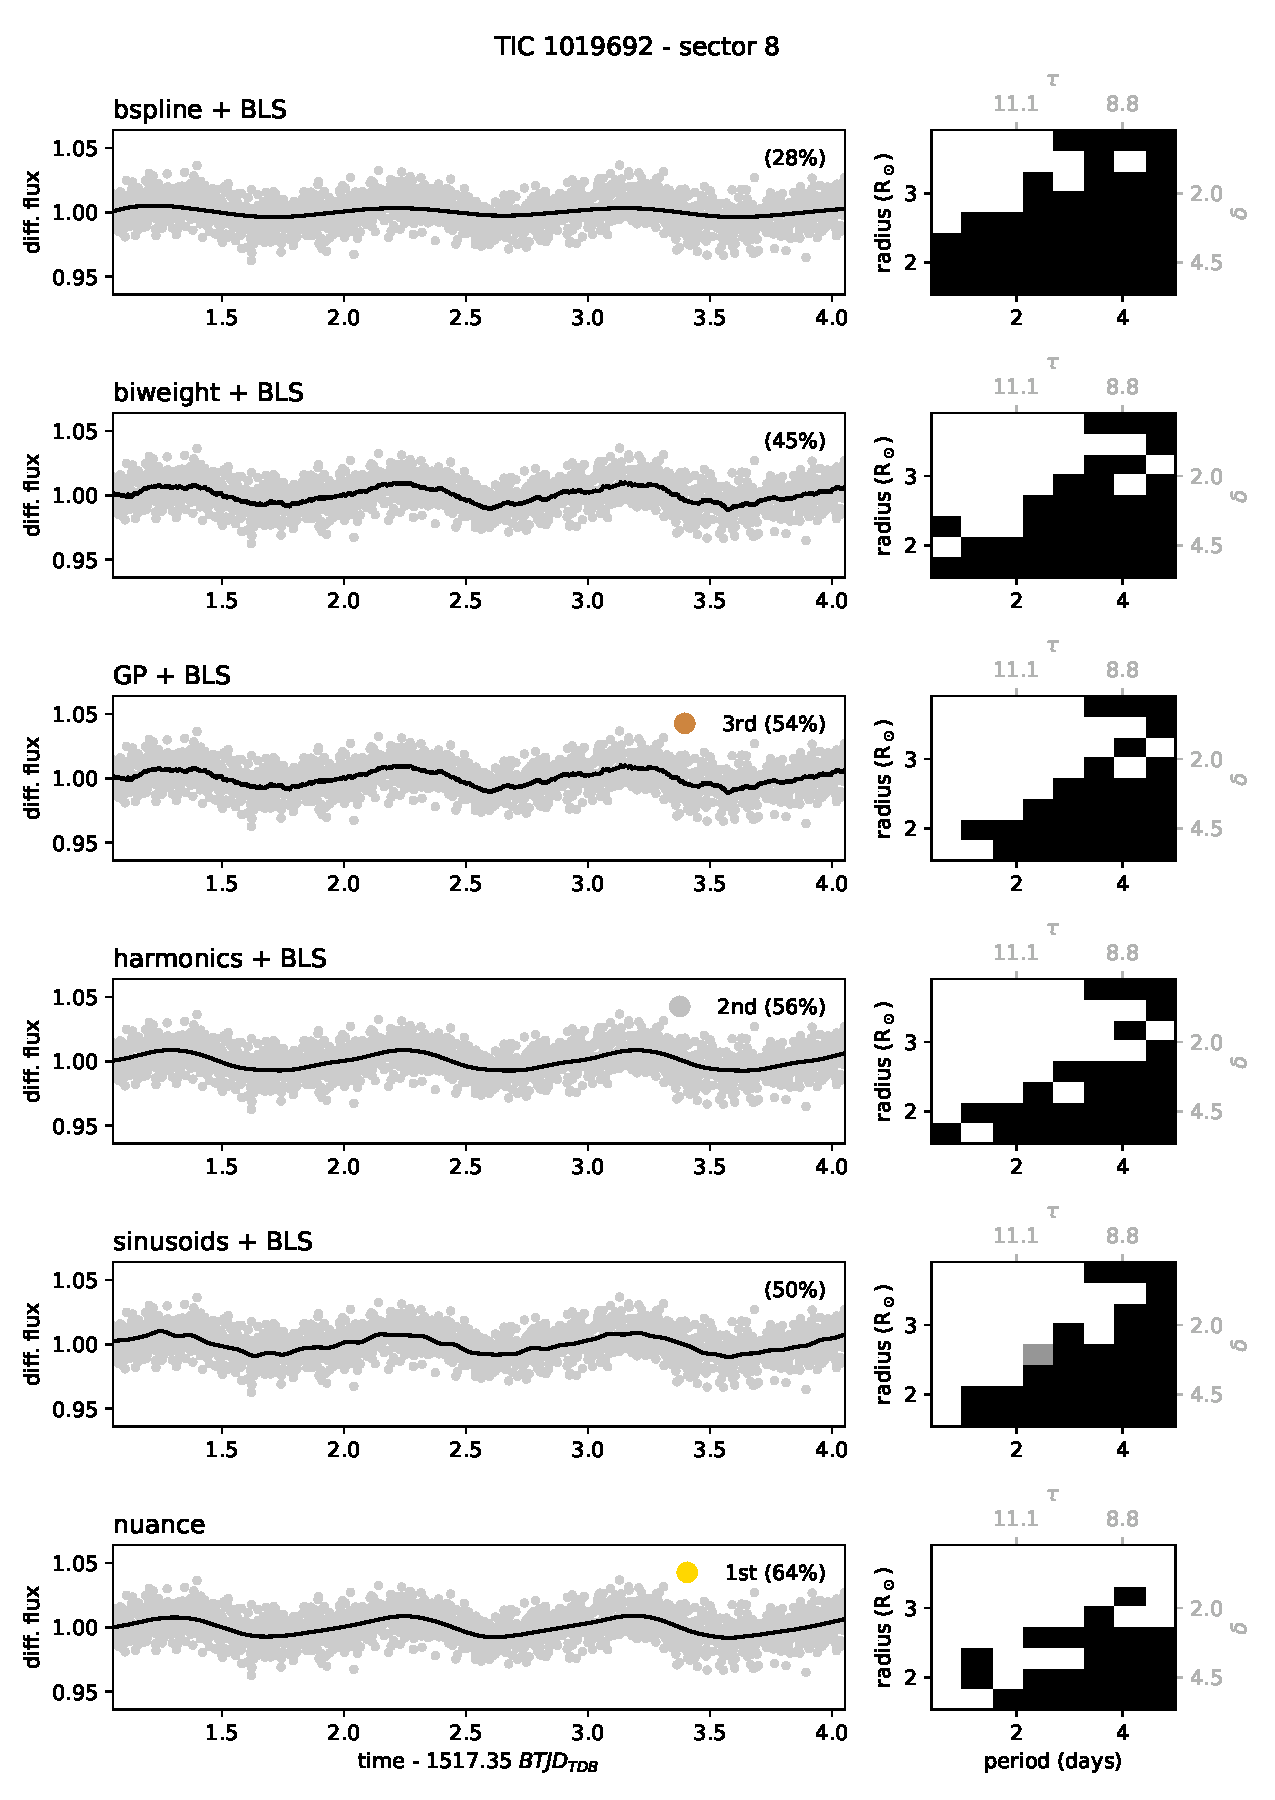
\includegraphics[width=\linewidth]{../workflows/tess_injection_recovery/figures/searched/1019692.pdf}
    \end{centering}
\end{figure}

\begin{figure}[H]
    \begin{centering}
        \caption{Results of the transits injection-recovery on TIC 1019692 half-sector light curve. Left: cleaned light curve with computed trend overplotted in black (except for \textsf{nuance} where it corresponds to the mean of the GP model). Right: Results of the transit search where a black square denotes a transit signal not detected, gray a signal detected at an alias period ($P/2$ or $2P$), and  white a signal detected with the correct period. On the right plots, secondary axes show the $(\tau, \delta)$ relative parameter space. For each method, the upper right legend on the left plot indicates its ranking based on the percent of recovered transit signals (where a transit with an aliased period counts as being detected).
        }
        \label{fig:onesearch}
    \end{centering}
\end{figure}


\bibliography{ref}

\end{document}